\vspace*{\fill}

\subsubsection*{Input: 1011}
\label{q2-1011}

\begin{figure}[ht]
  \centering
  \begin{minipage}{.49\linewidth}
    \centering
    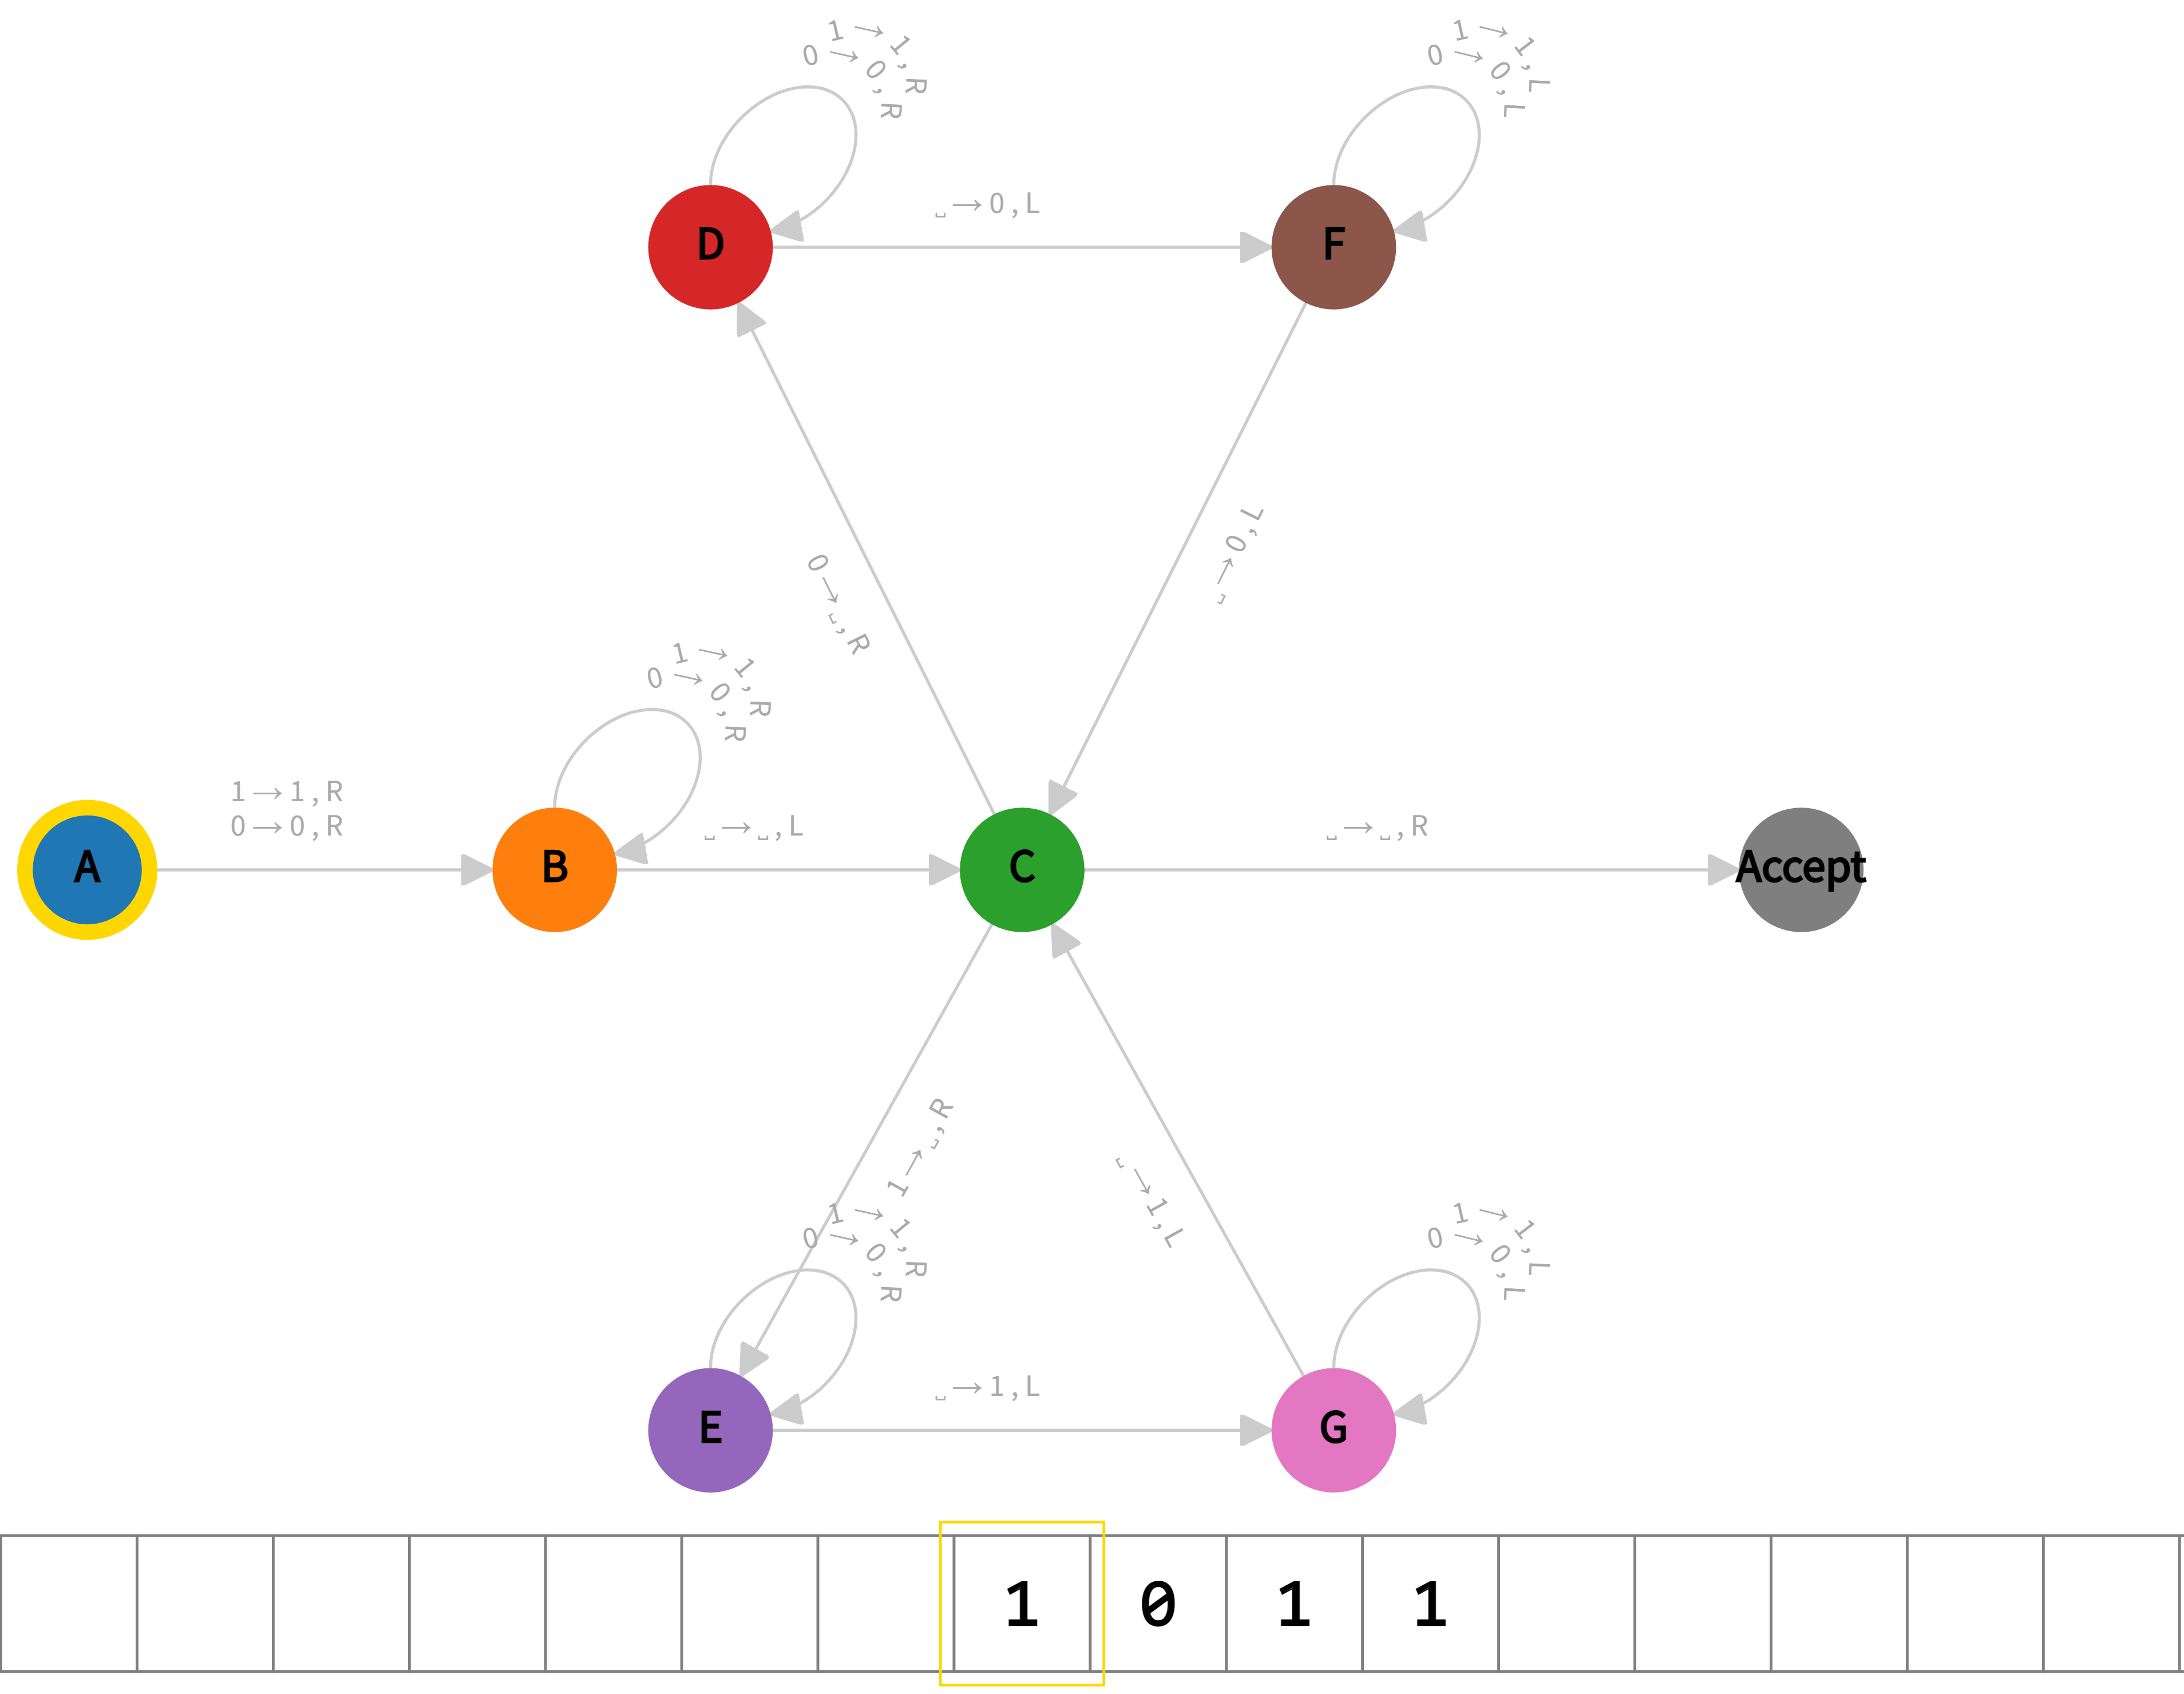
\includegraphics[width=\linewidth]{answers/img/q2-1011-initial.png}
    \caption*{Figure (a): Initial State for $\mathbf{1011}$}
    \label{fig:1011-initial}
  \end{minipage}
  \begin{minipage}{.49\linewidth}
    \centering
    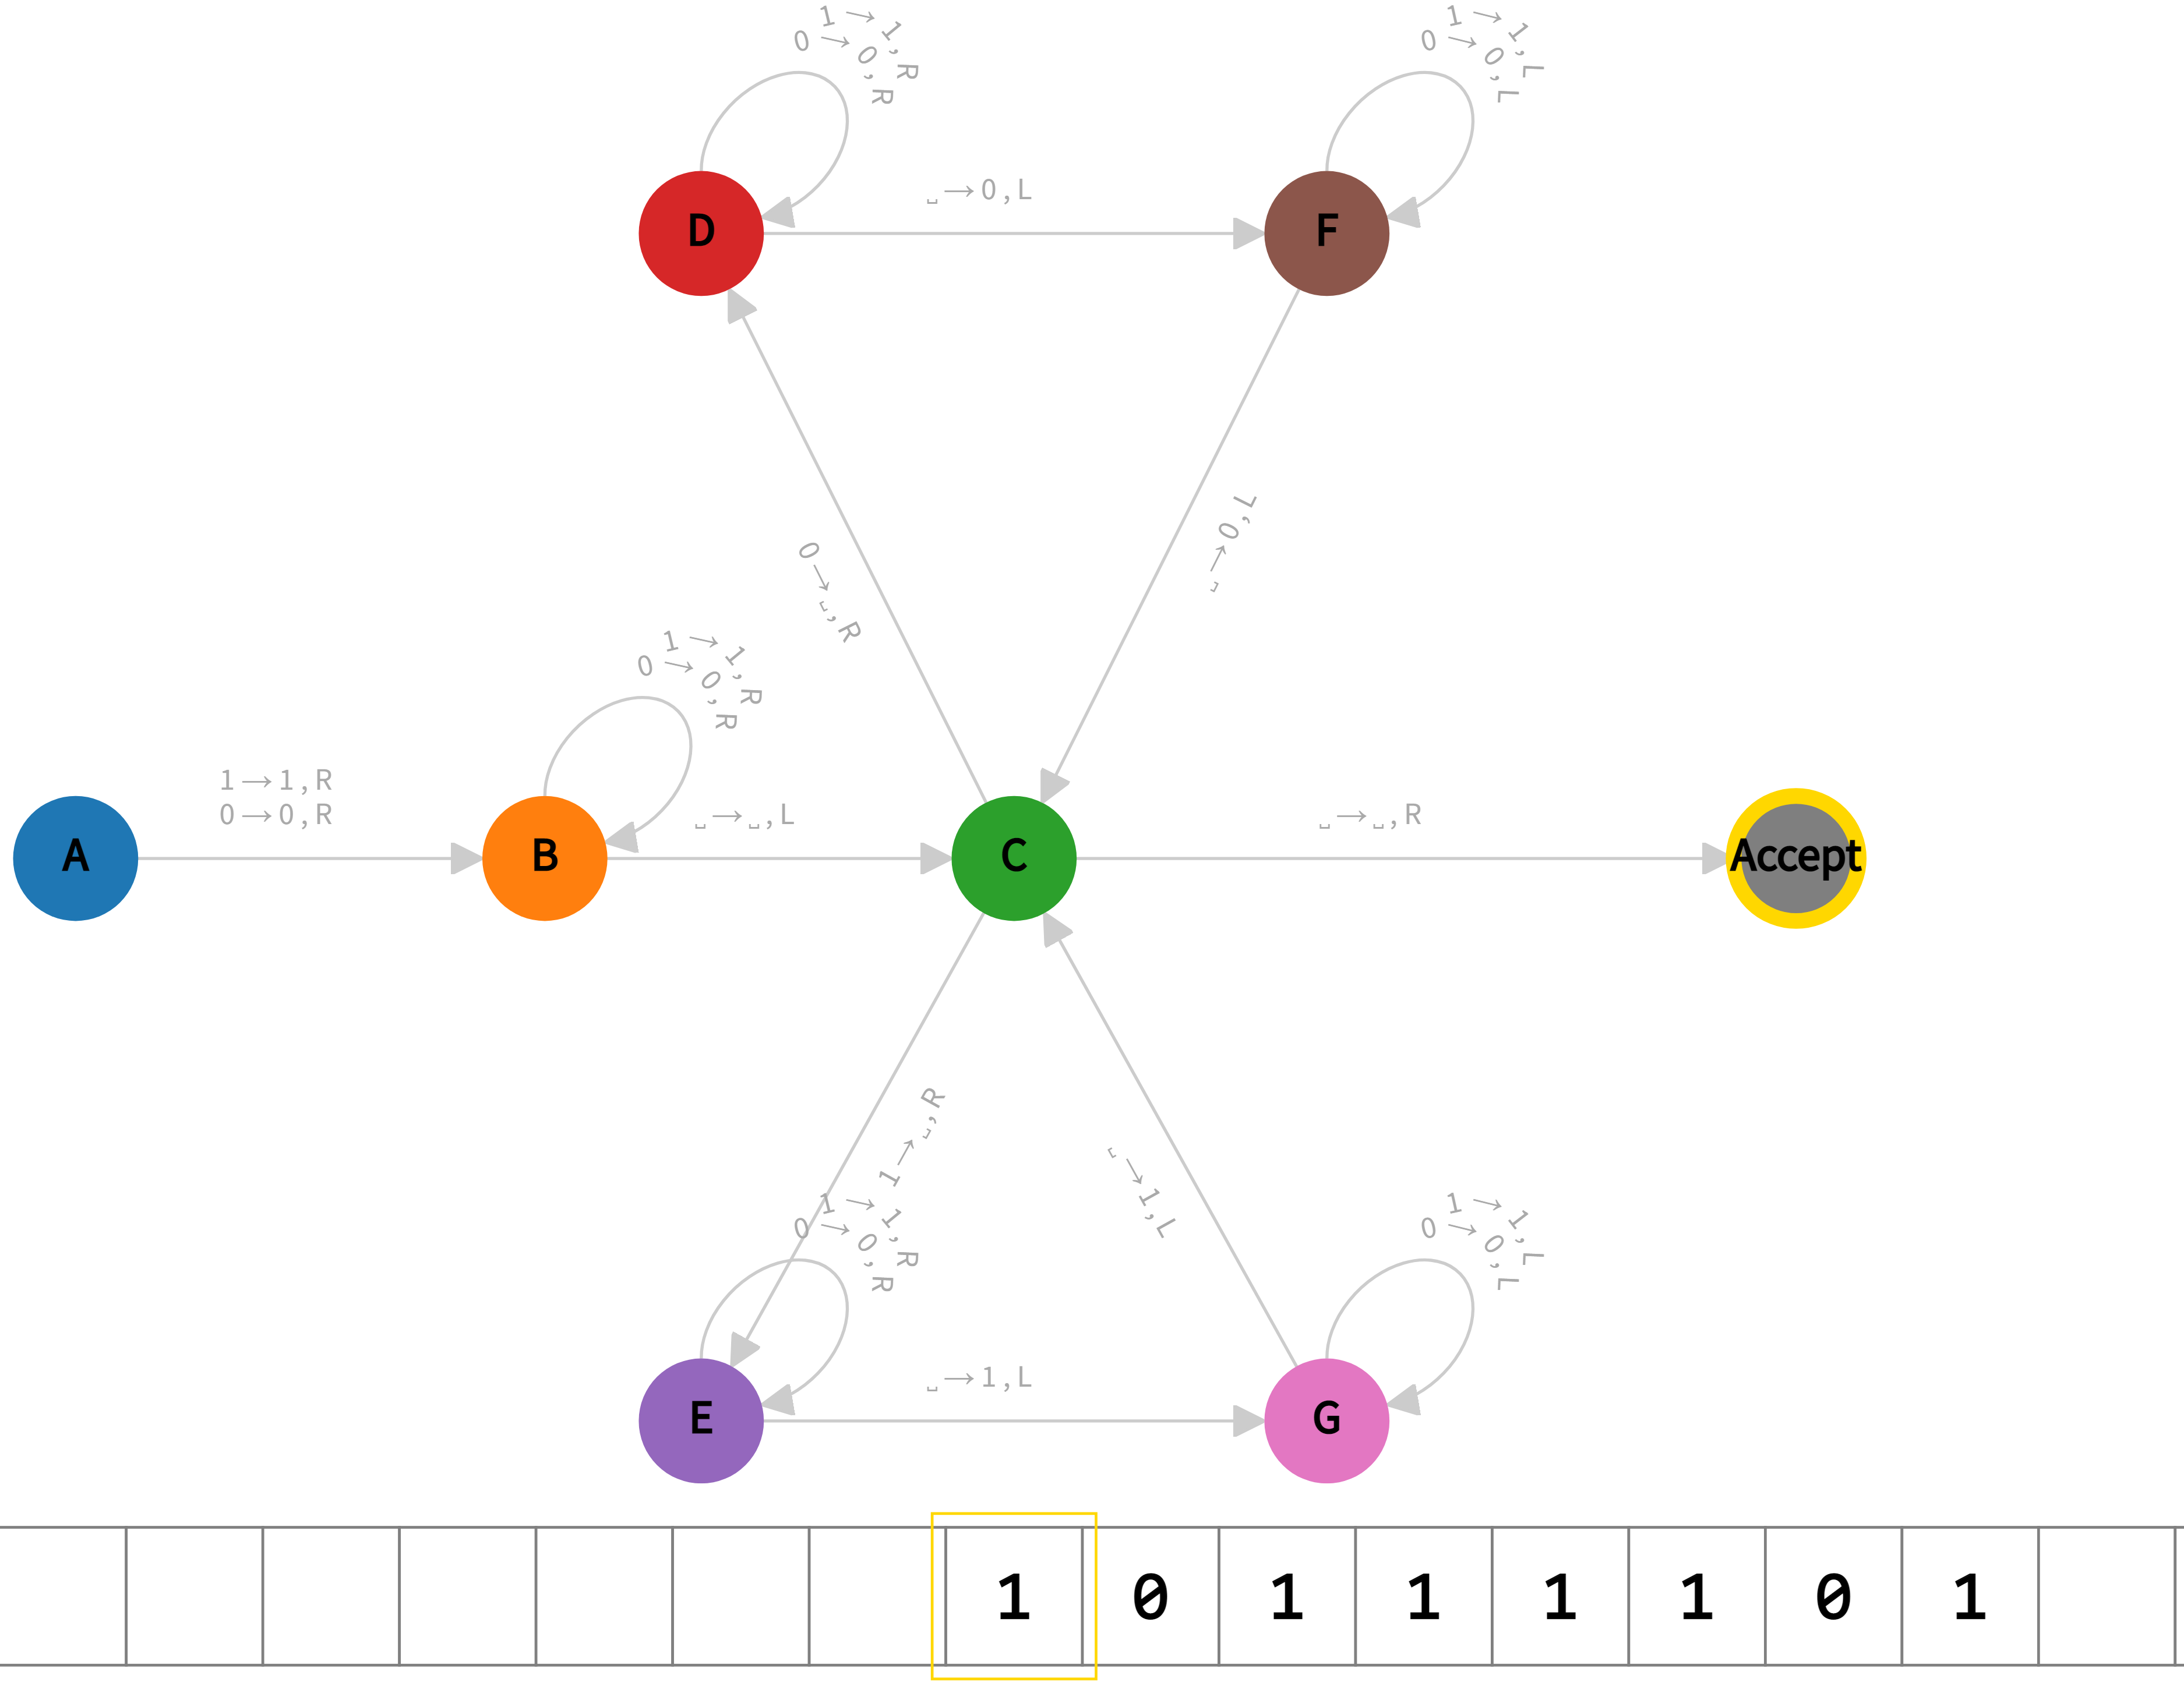
\includegraphics[width=\linewidth]{answers/img/q2-1011-end.png}
    \caption*{Figure (b): End State for $\mathbf{1011}$}
    \label{fig:1011-end}
  \end{minipage}
  \caption{States for $\mathbf{1011}$}
  \label{fig:in-1011}
\end{figure}

\subsubsection*{Input: 1110}
\label{q2-1110}

\begin{figure}[ht]
  \centering
  \begin{minipage}{.49\linewidth}
    \centering
    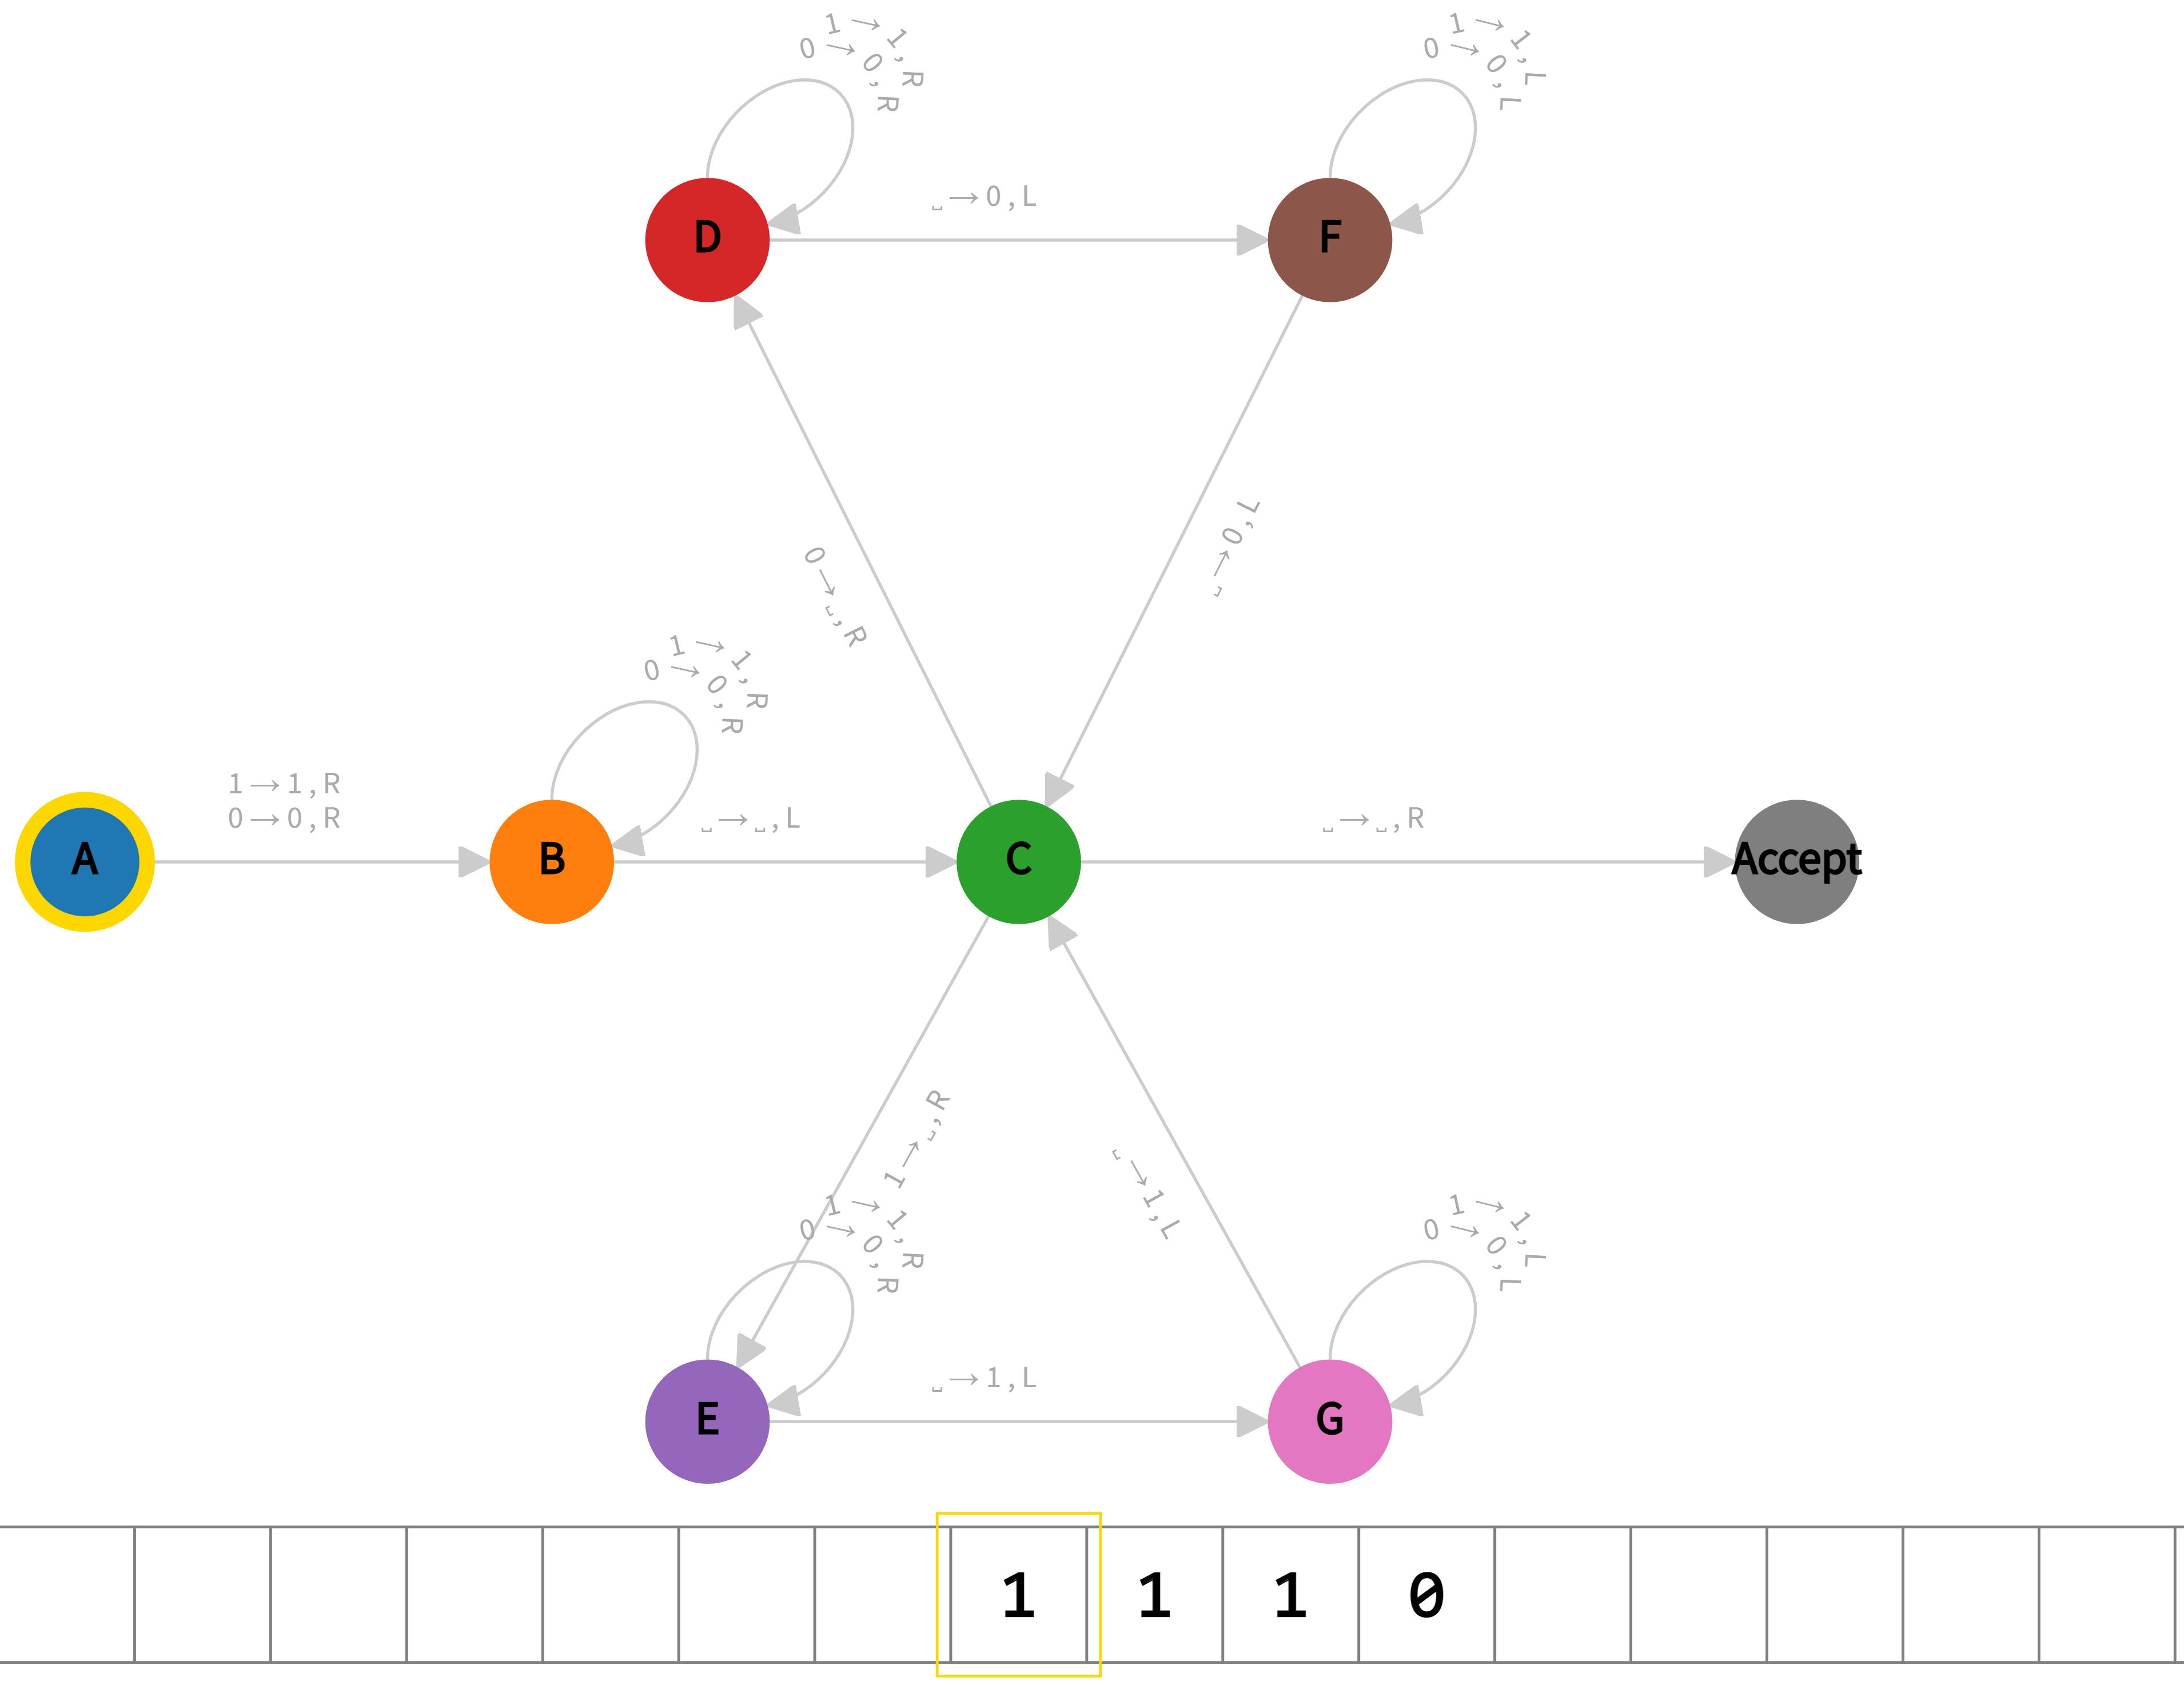
\includegraphics[width=\linewidth]{answers/img/q2-1110-initial.png}
    \caption*{Figure (a): Initial State for $\mathbf{1110}$}
    \label{fig:1110-initial}
  \end{minipage}
  \begin{minipage}{.49\linewidth}
    \centering
    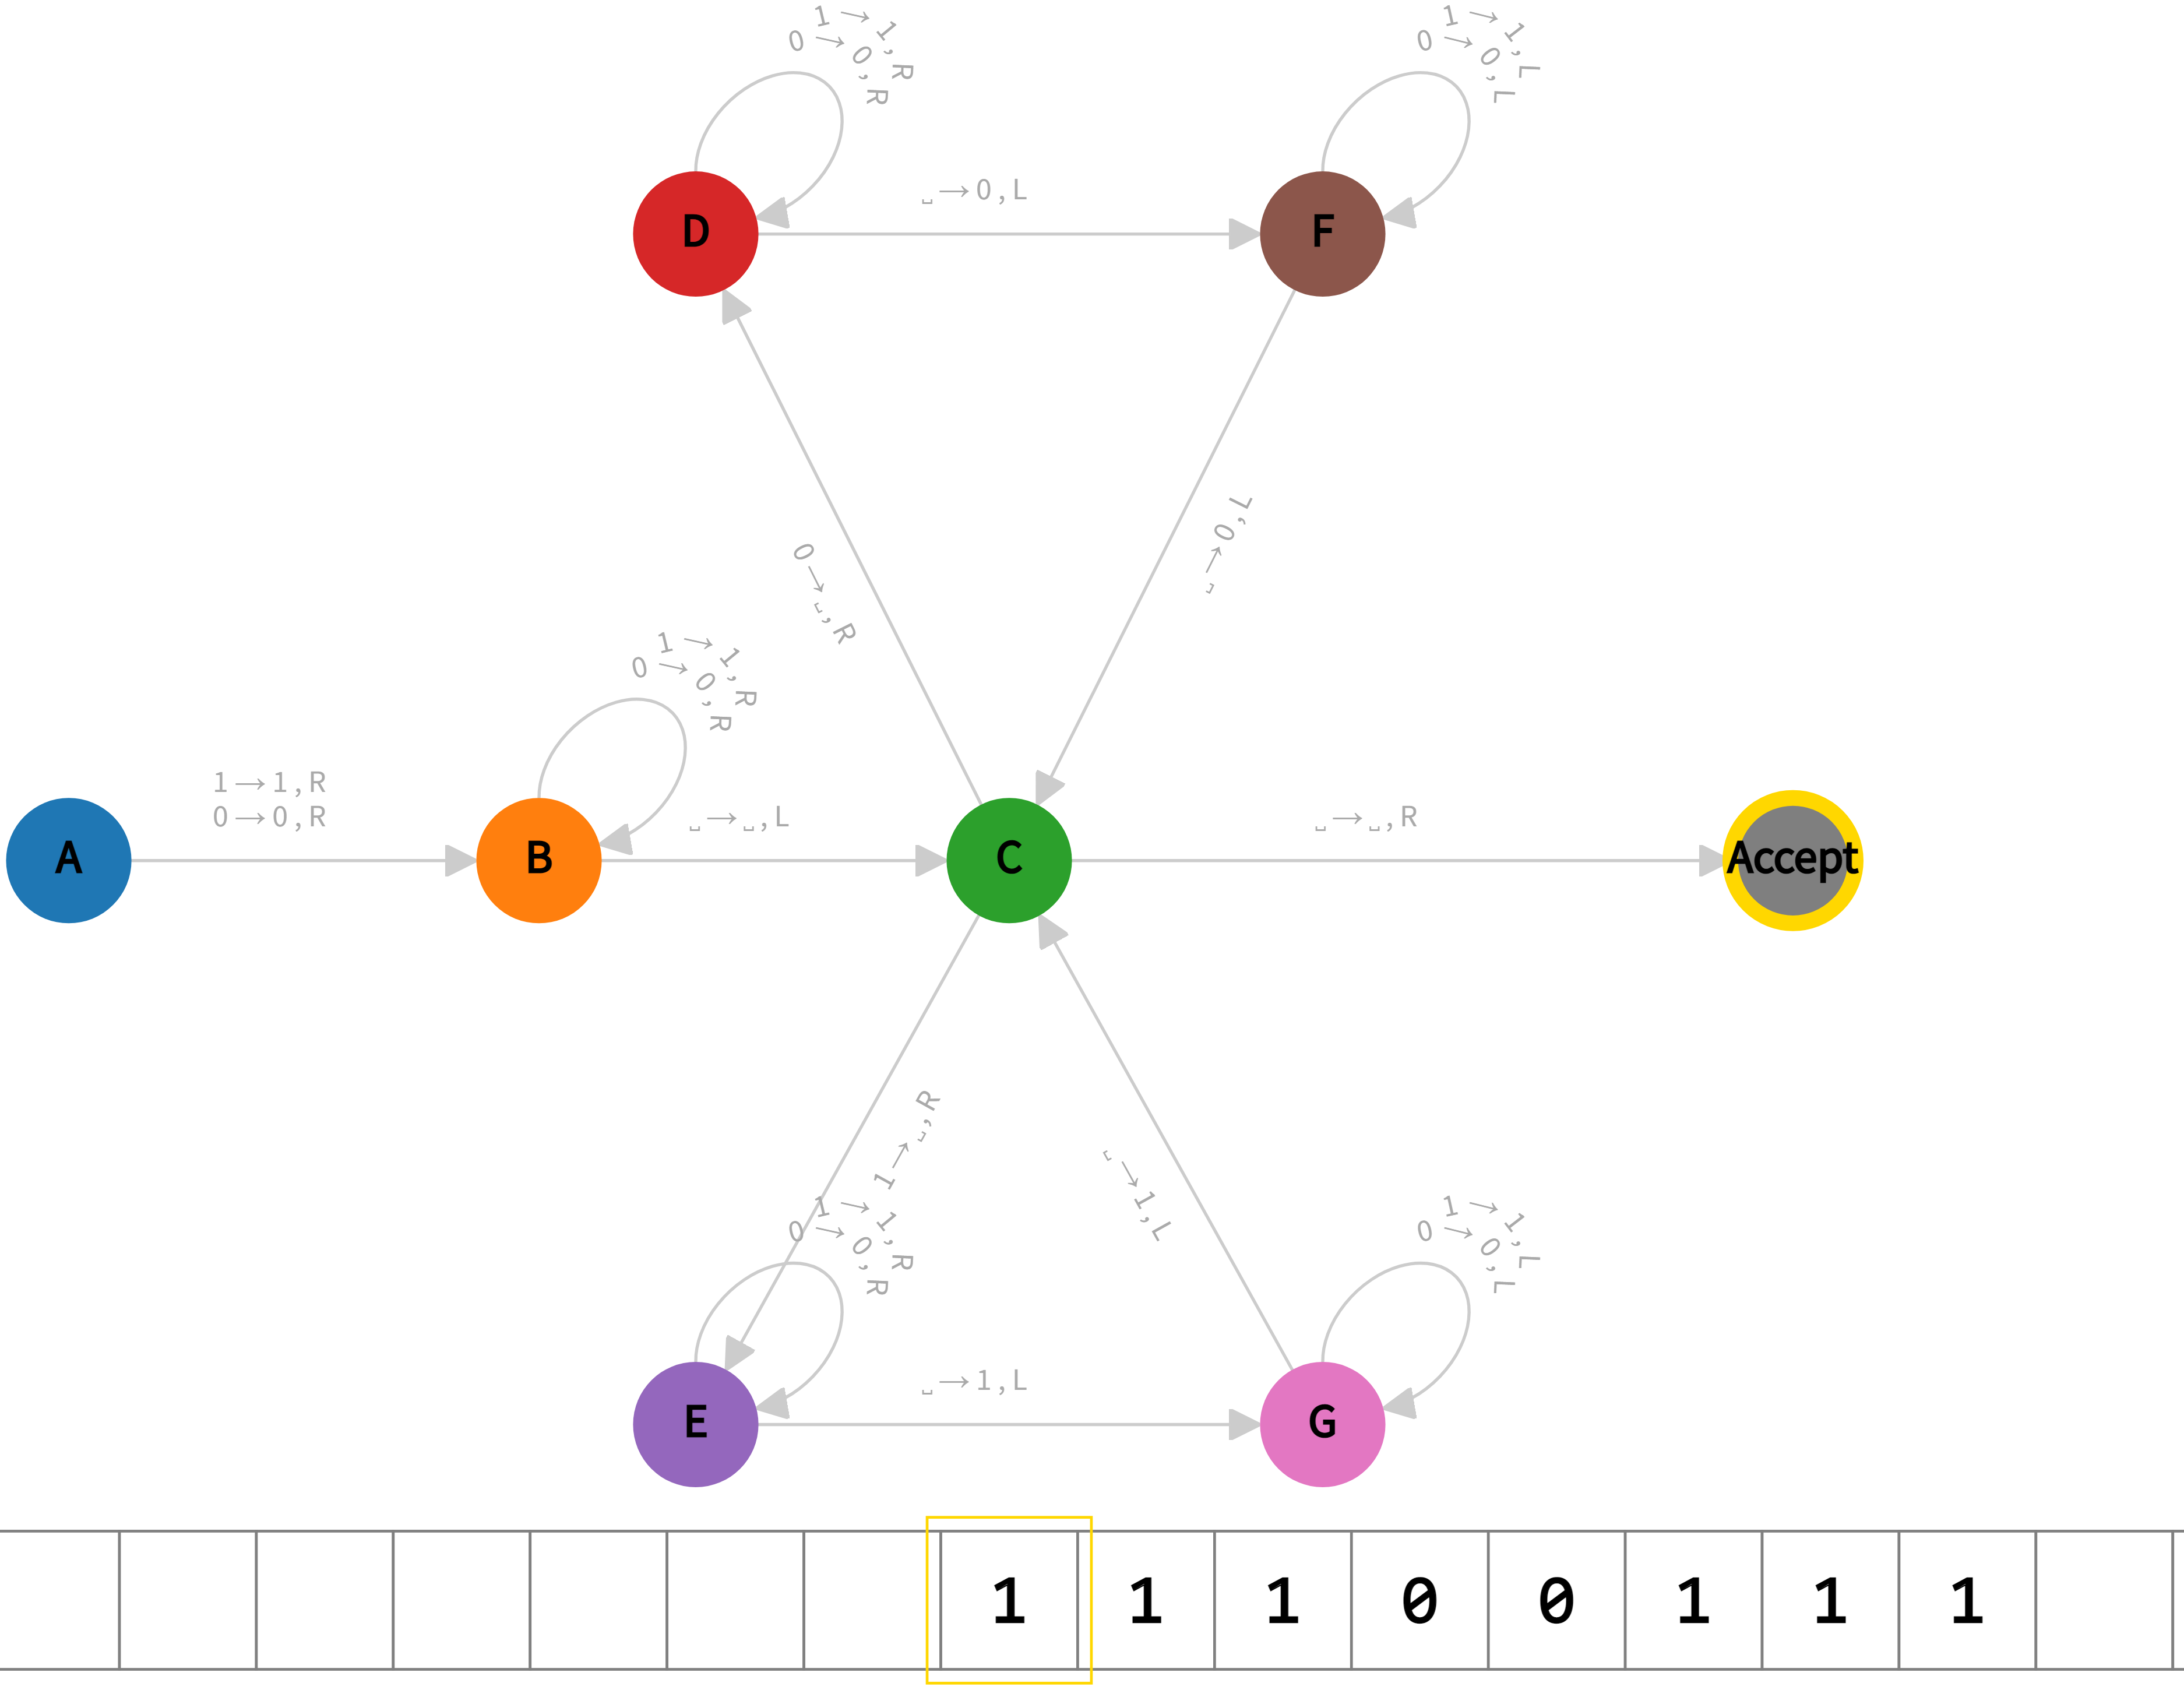
\includegraphics[width=\linewidth]{answers/img/q2-1110-end.png}
    \caption*{Figure (b): End State for $\mathbf{1110}$}
    \label{fig:1110-end}
  \end{minipage}
  \caption{States for $\mathbf{1110}$}
  \label{fig:in-1110}
\end{figure}

\vspace*{\fill}

\newpage

\vspace*{\fill}

\subsubsection*{Input: 0101}
\label{q2-0101}

\begin{figure}[ht]
  \centering
  \begin{minipage}{.49\linewidth}
    \centering
    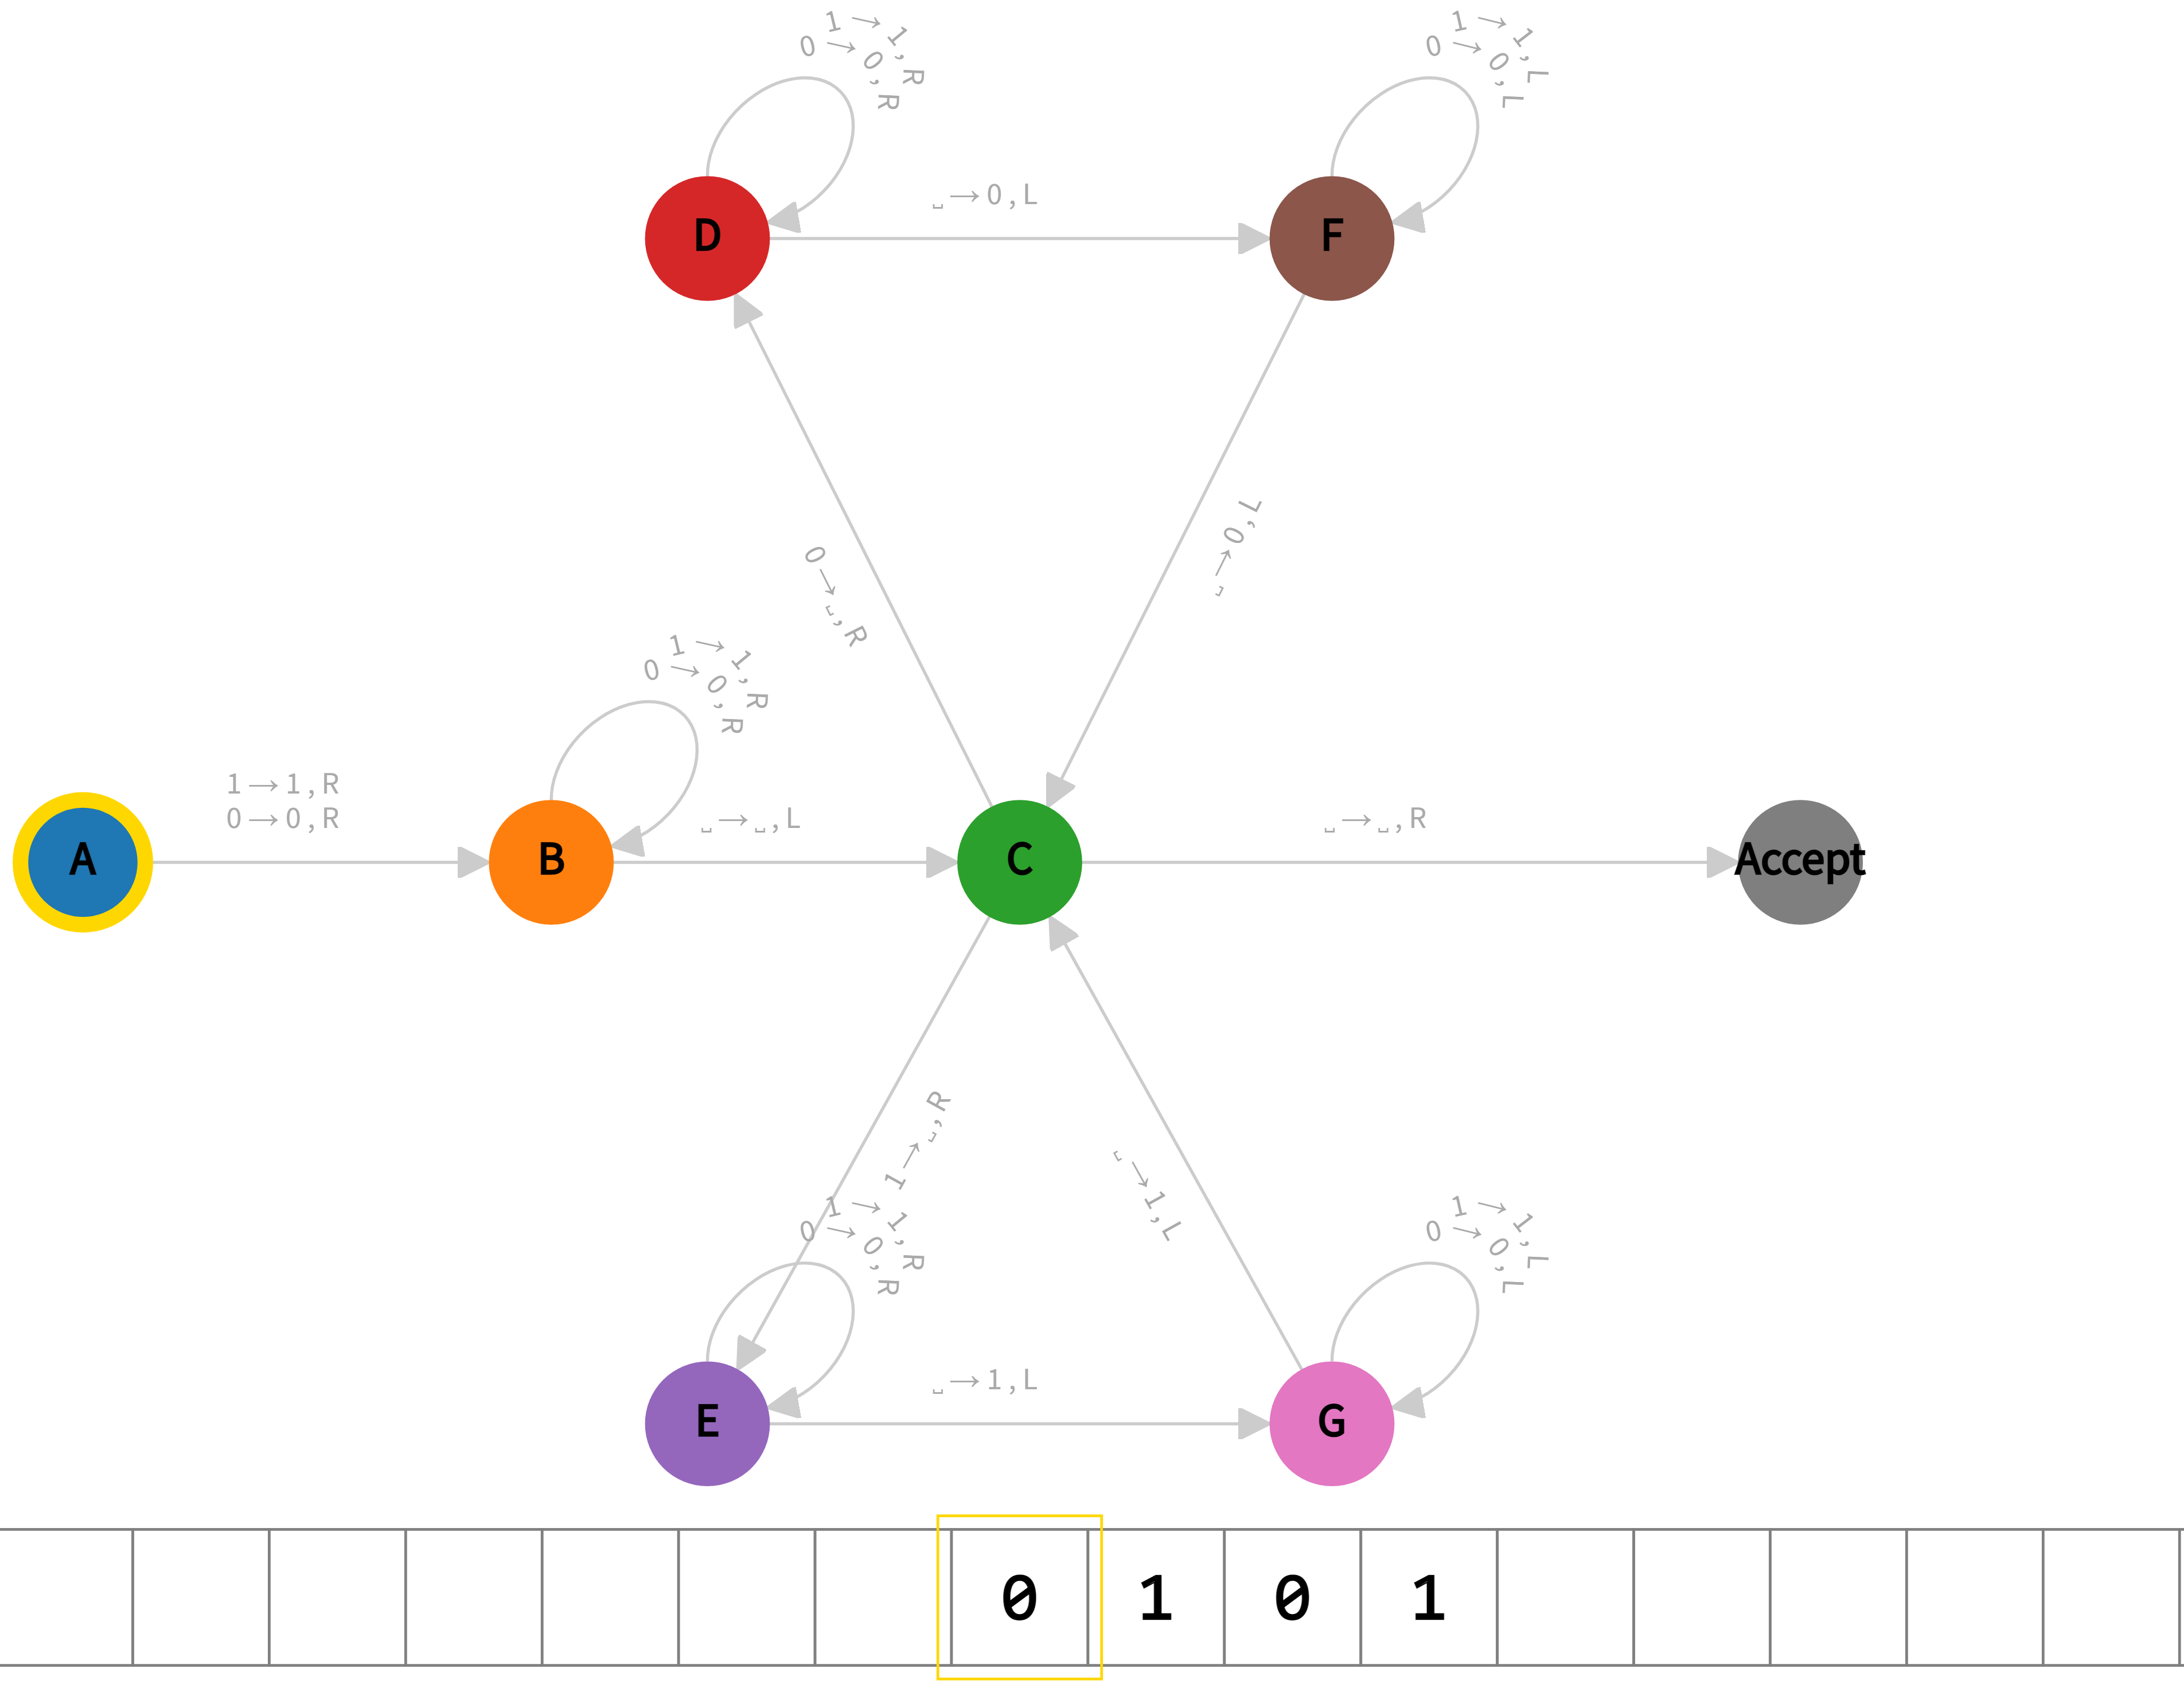
\includegraphics[width=\linewidth]{answers/img/q2-0101-initial.png}
    \caption*{Figure (a): Initial State for $\mathbf{0101}$}
    \label{fig:0101-initial}
  \end{minipage}
  \begin{minipage}{.49\linewidth}
    \centering
    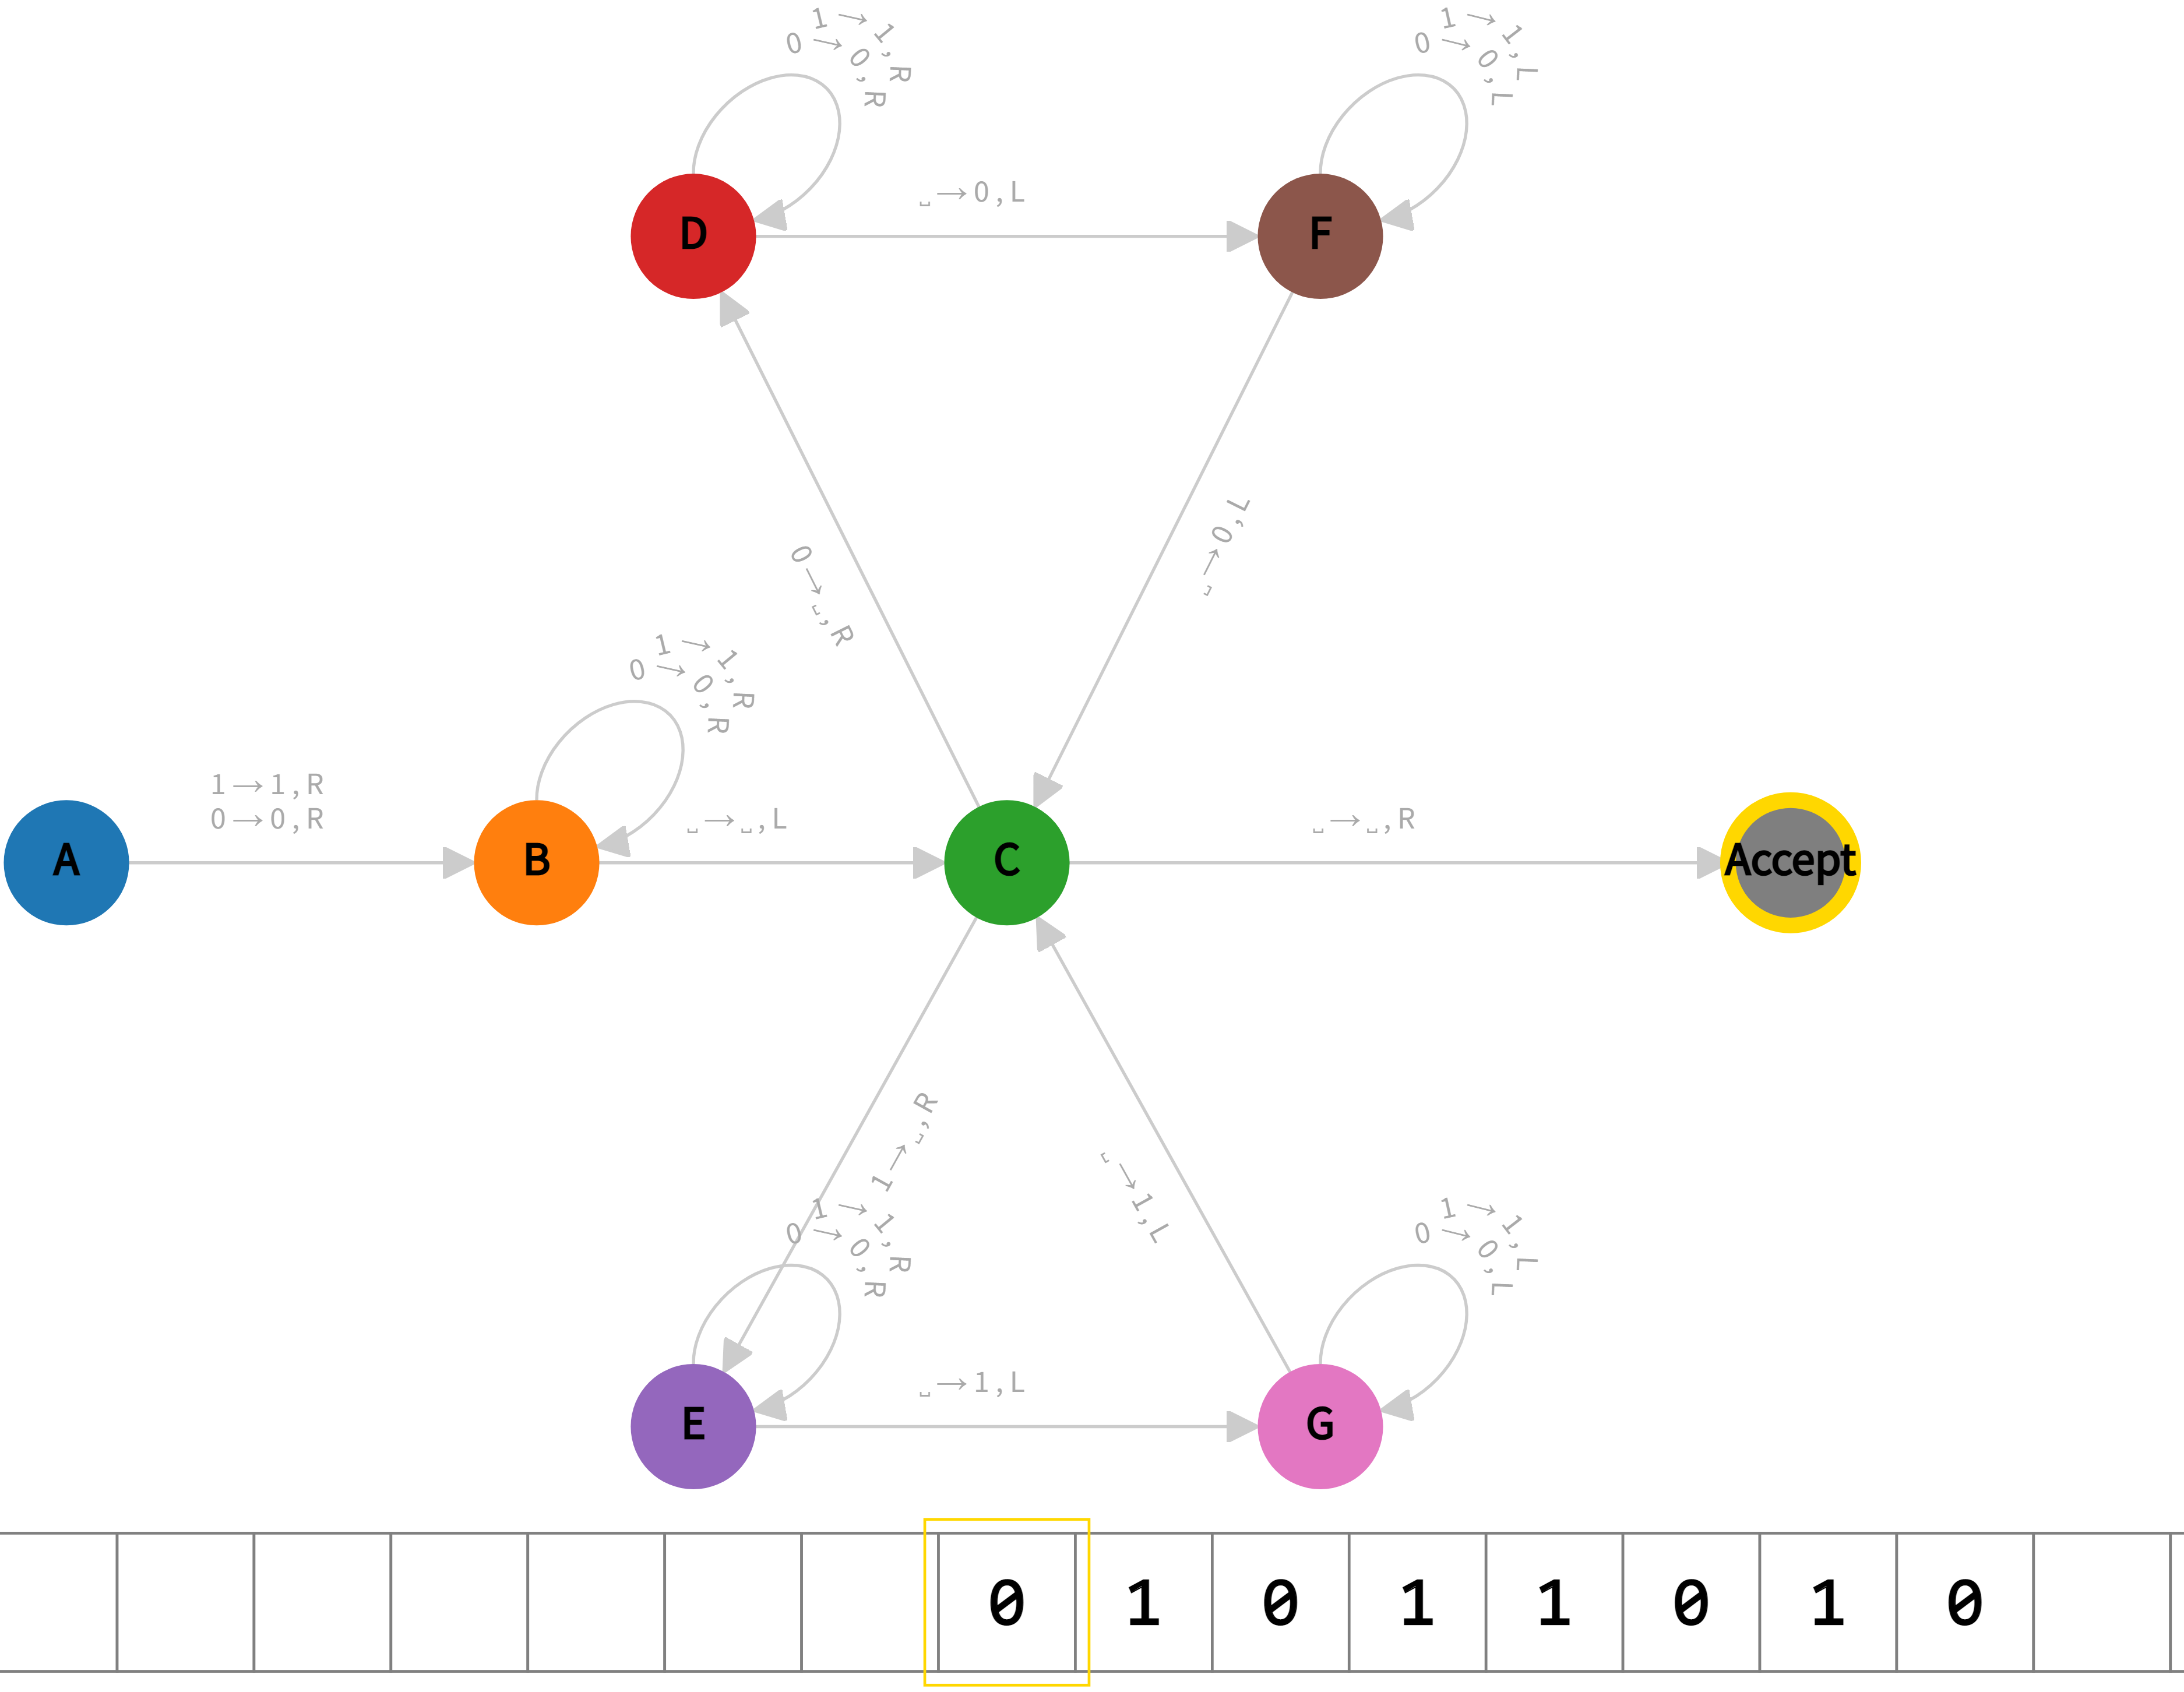
\includegraphics[width=\linewidth]{answers/img/q2-0101-end.png}
    \caption*{Figure (b): End State for $\mathbf{0101}$}
    \label{fig:0101-end}
  \end{minipage}
  \caption{States for $\mathbf{0101}$}
  \label{fig:in-0101}
\end{figure}

\subsubsection*{Input: 1010}
\label{q2-1010}

\begin{figure}[ht]
  \centering
  \begin{minipage}{.49\linewidth}
    \centering
    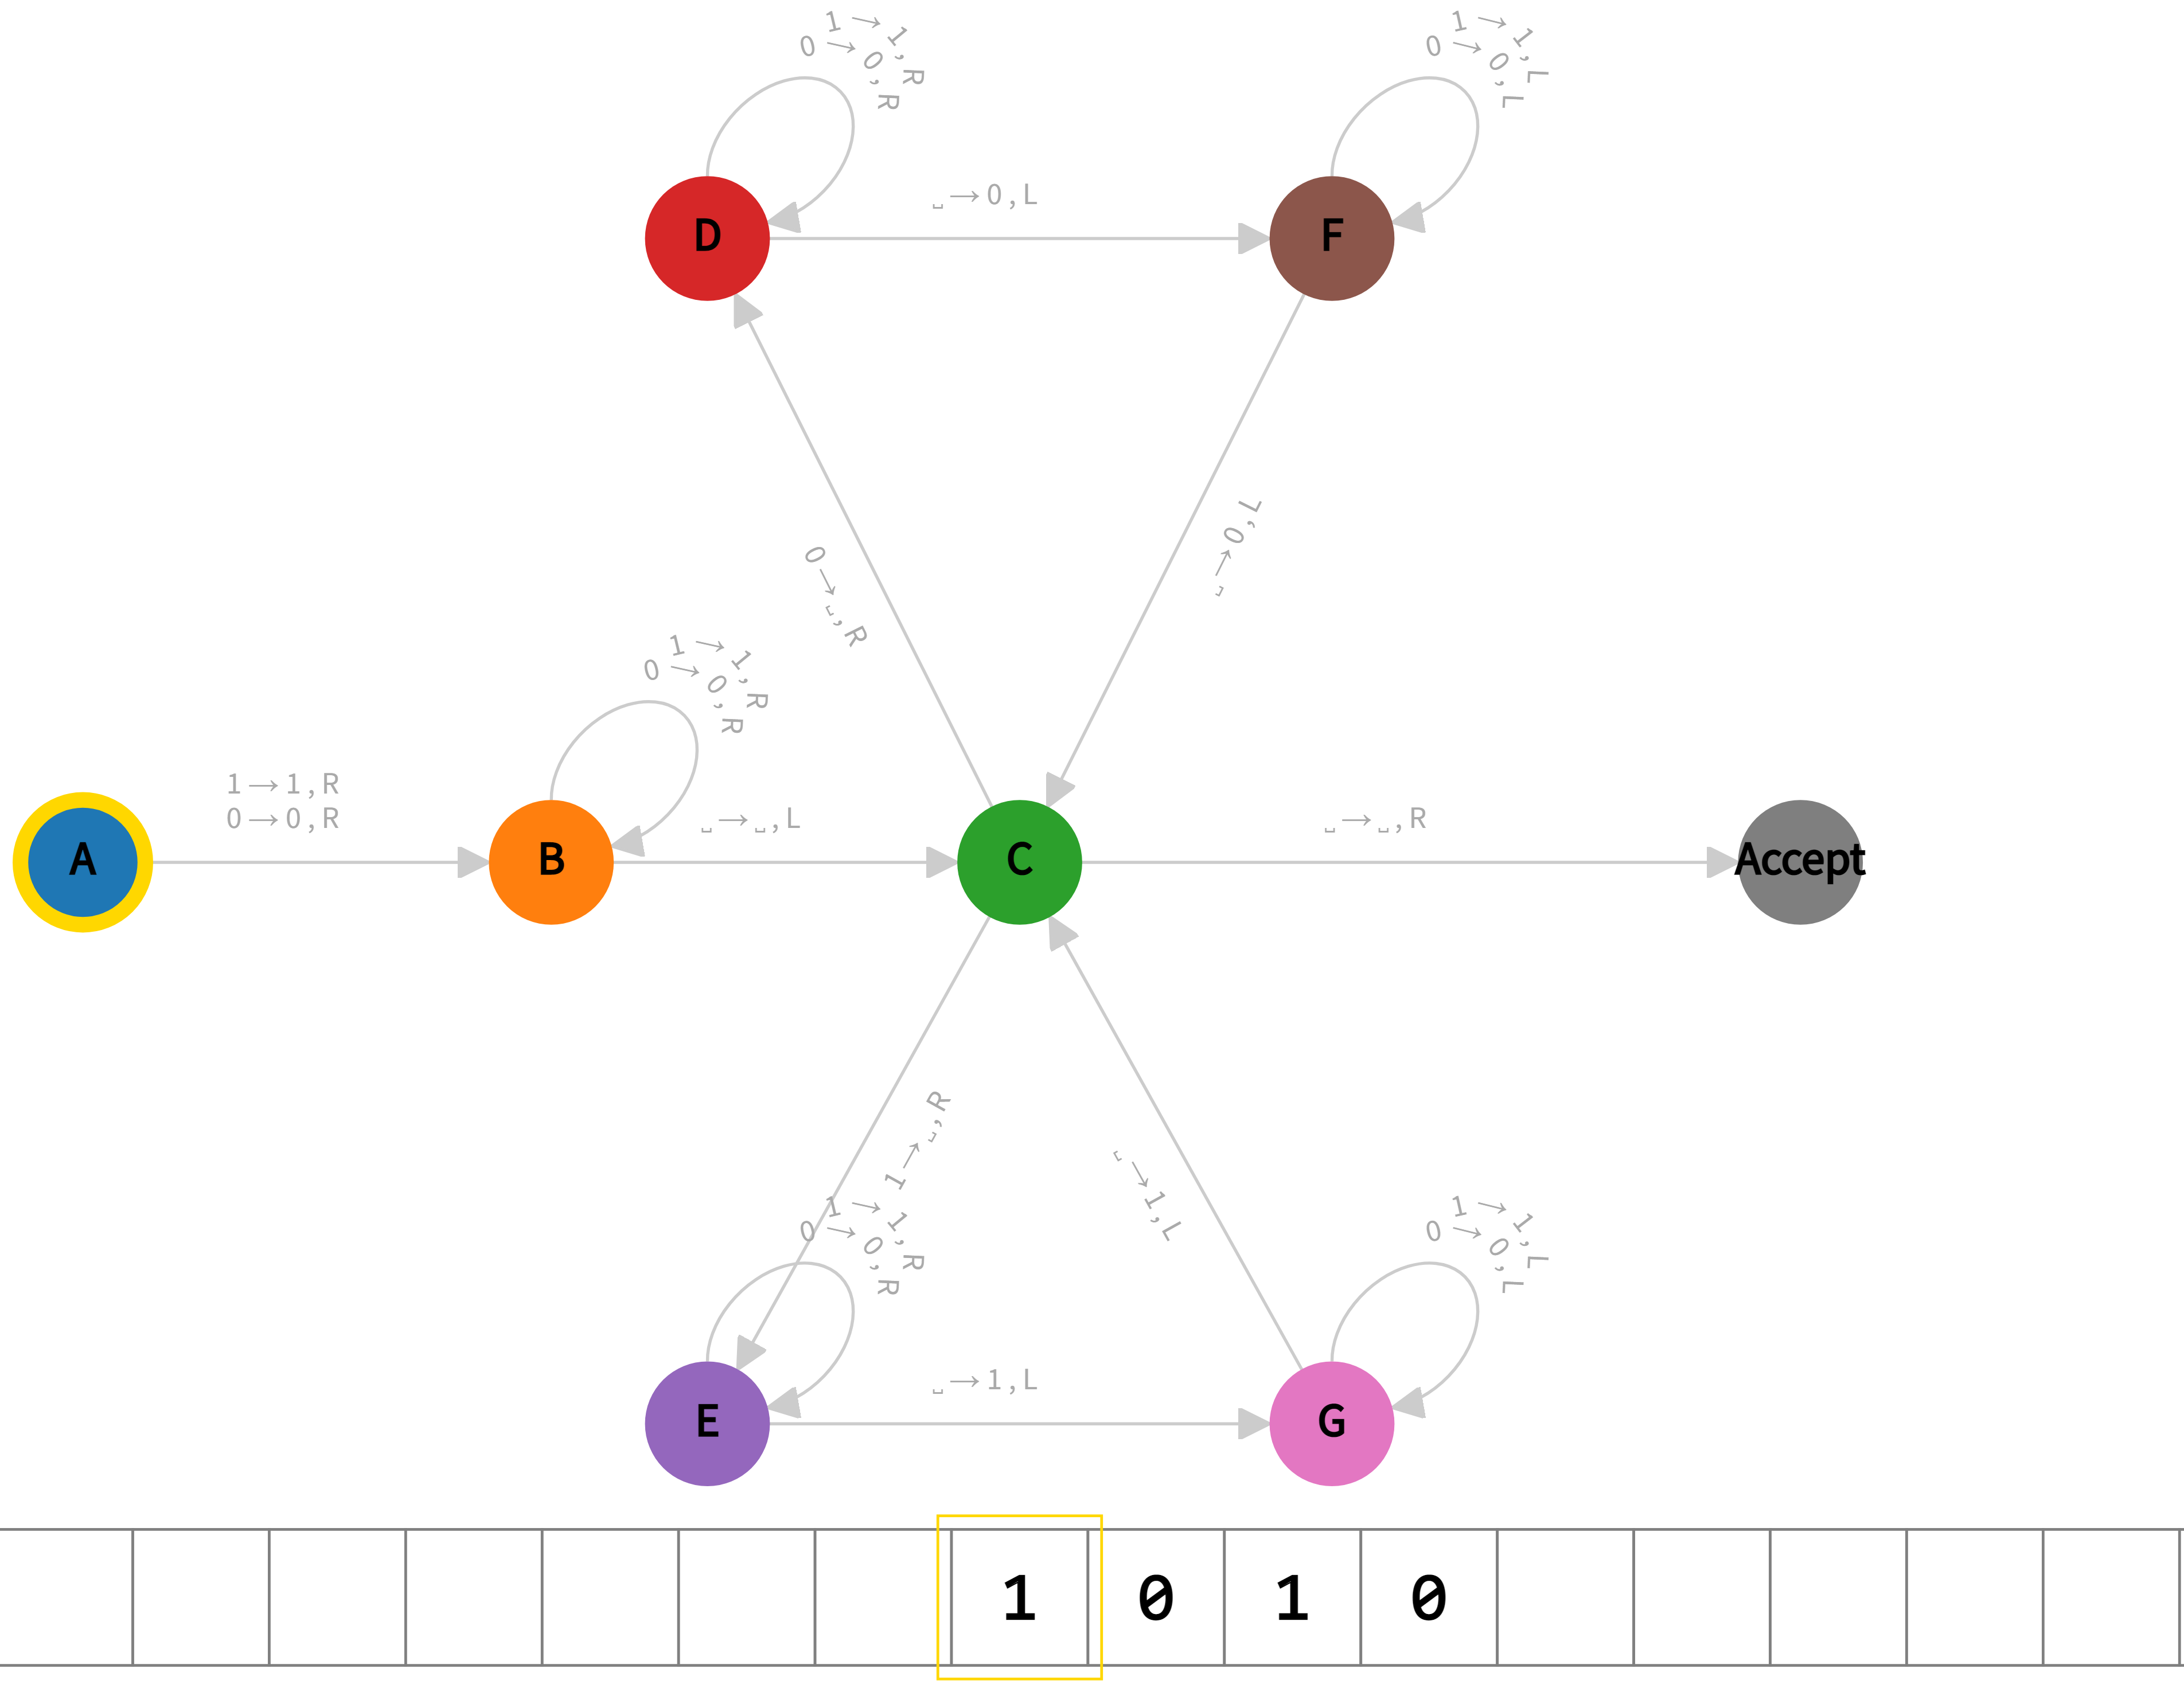
\includegraphics[width=\linewidth]{answers/img/q2-1010-initial.png}
    \caption*{Figure (a): Initial State for $\mathbf{1010}$}
    \label{fig:1010-initial}
  \end{minipage}
  \begin{minipage}{.49\linewidth}
    \centering
    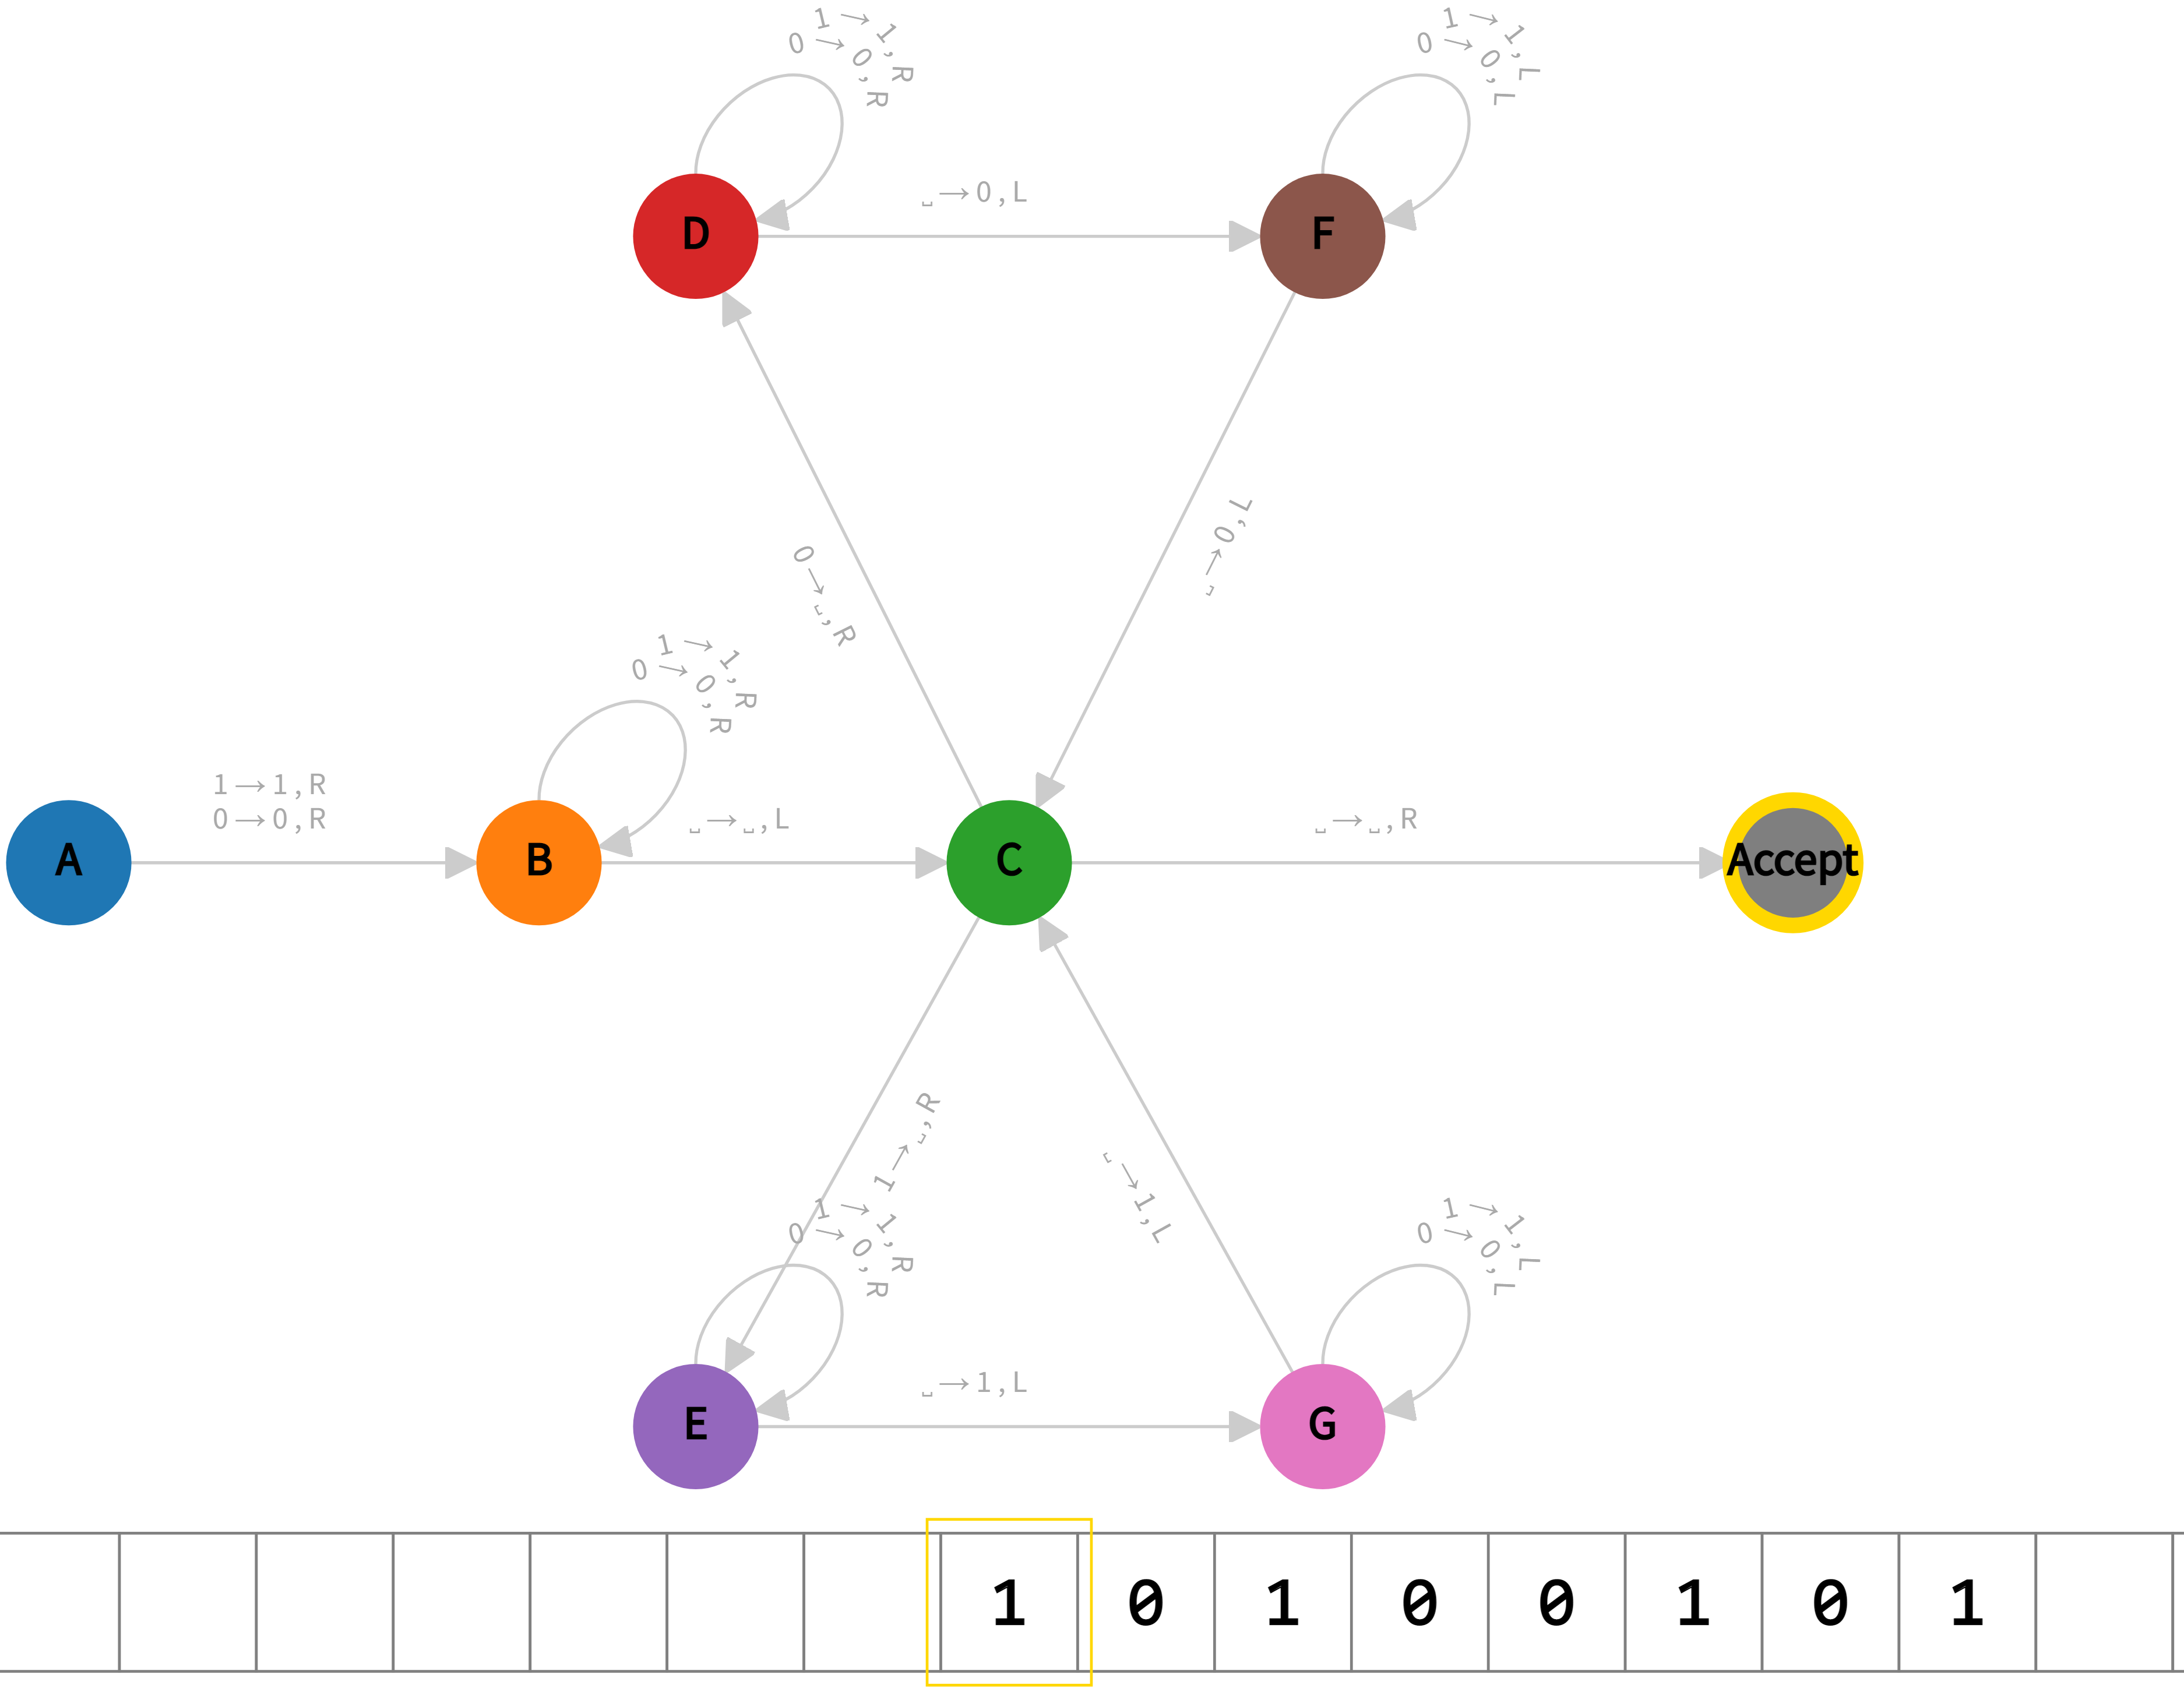
\includegraphics[width=\linewidth]{answers/img/q2-1010-end.png}
    \caption*{Figure (b): End State for $\mathbf{1010}$}
    \label{fig:1010-end}
  \end{minipage}
  \caption{States for $\mathbf{1010}$}
  \label{fig:in-1010}
\end{figure}

\vspace*{\fill}
\newpage
\vspace*{\fill}

\subsection*{Input: 1010001}

\begin{figure}[ht]
  \centering
  \begin{minipage}{.49\linewidth}
    \centering
    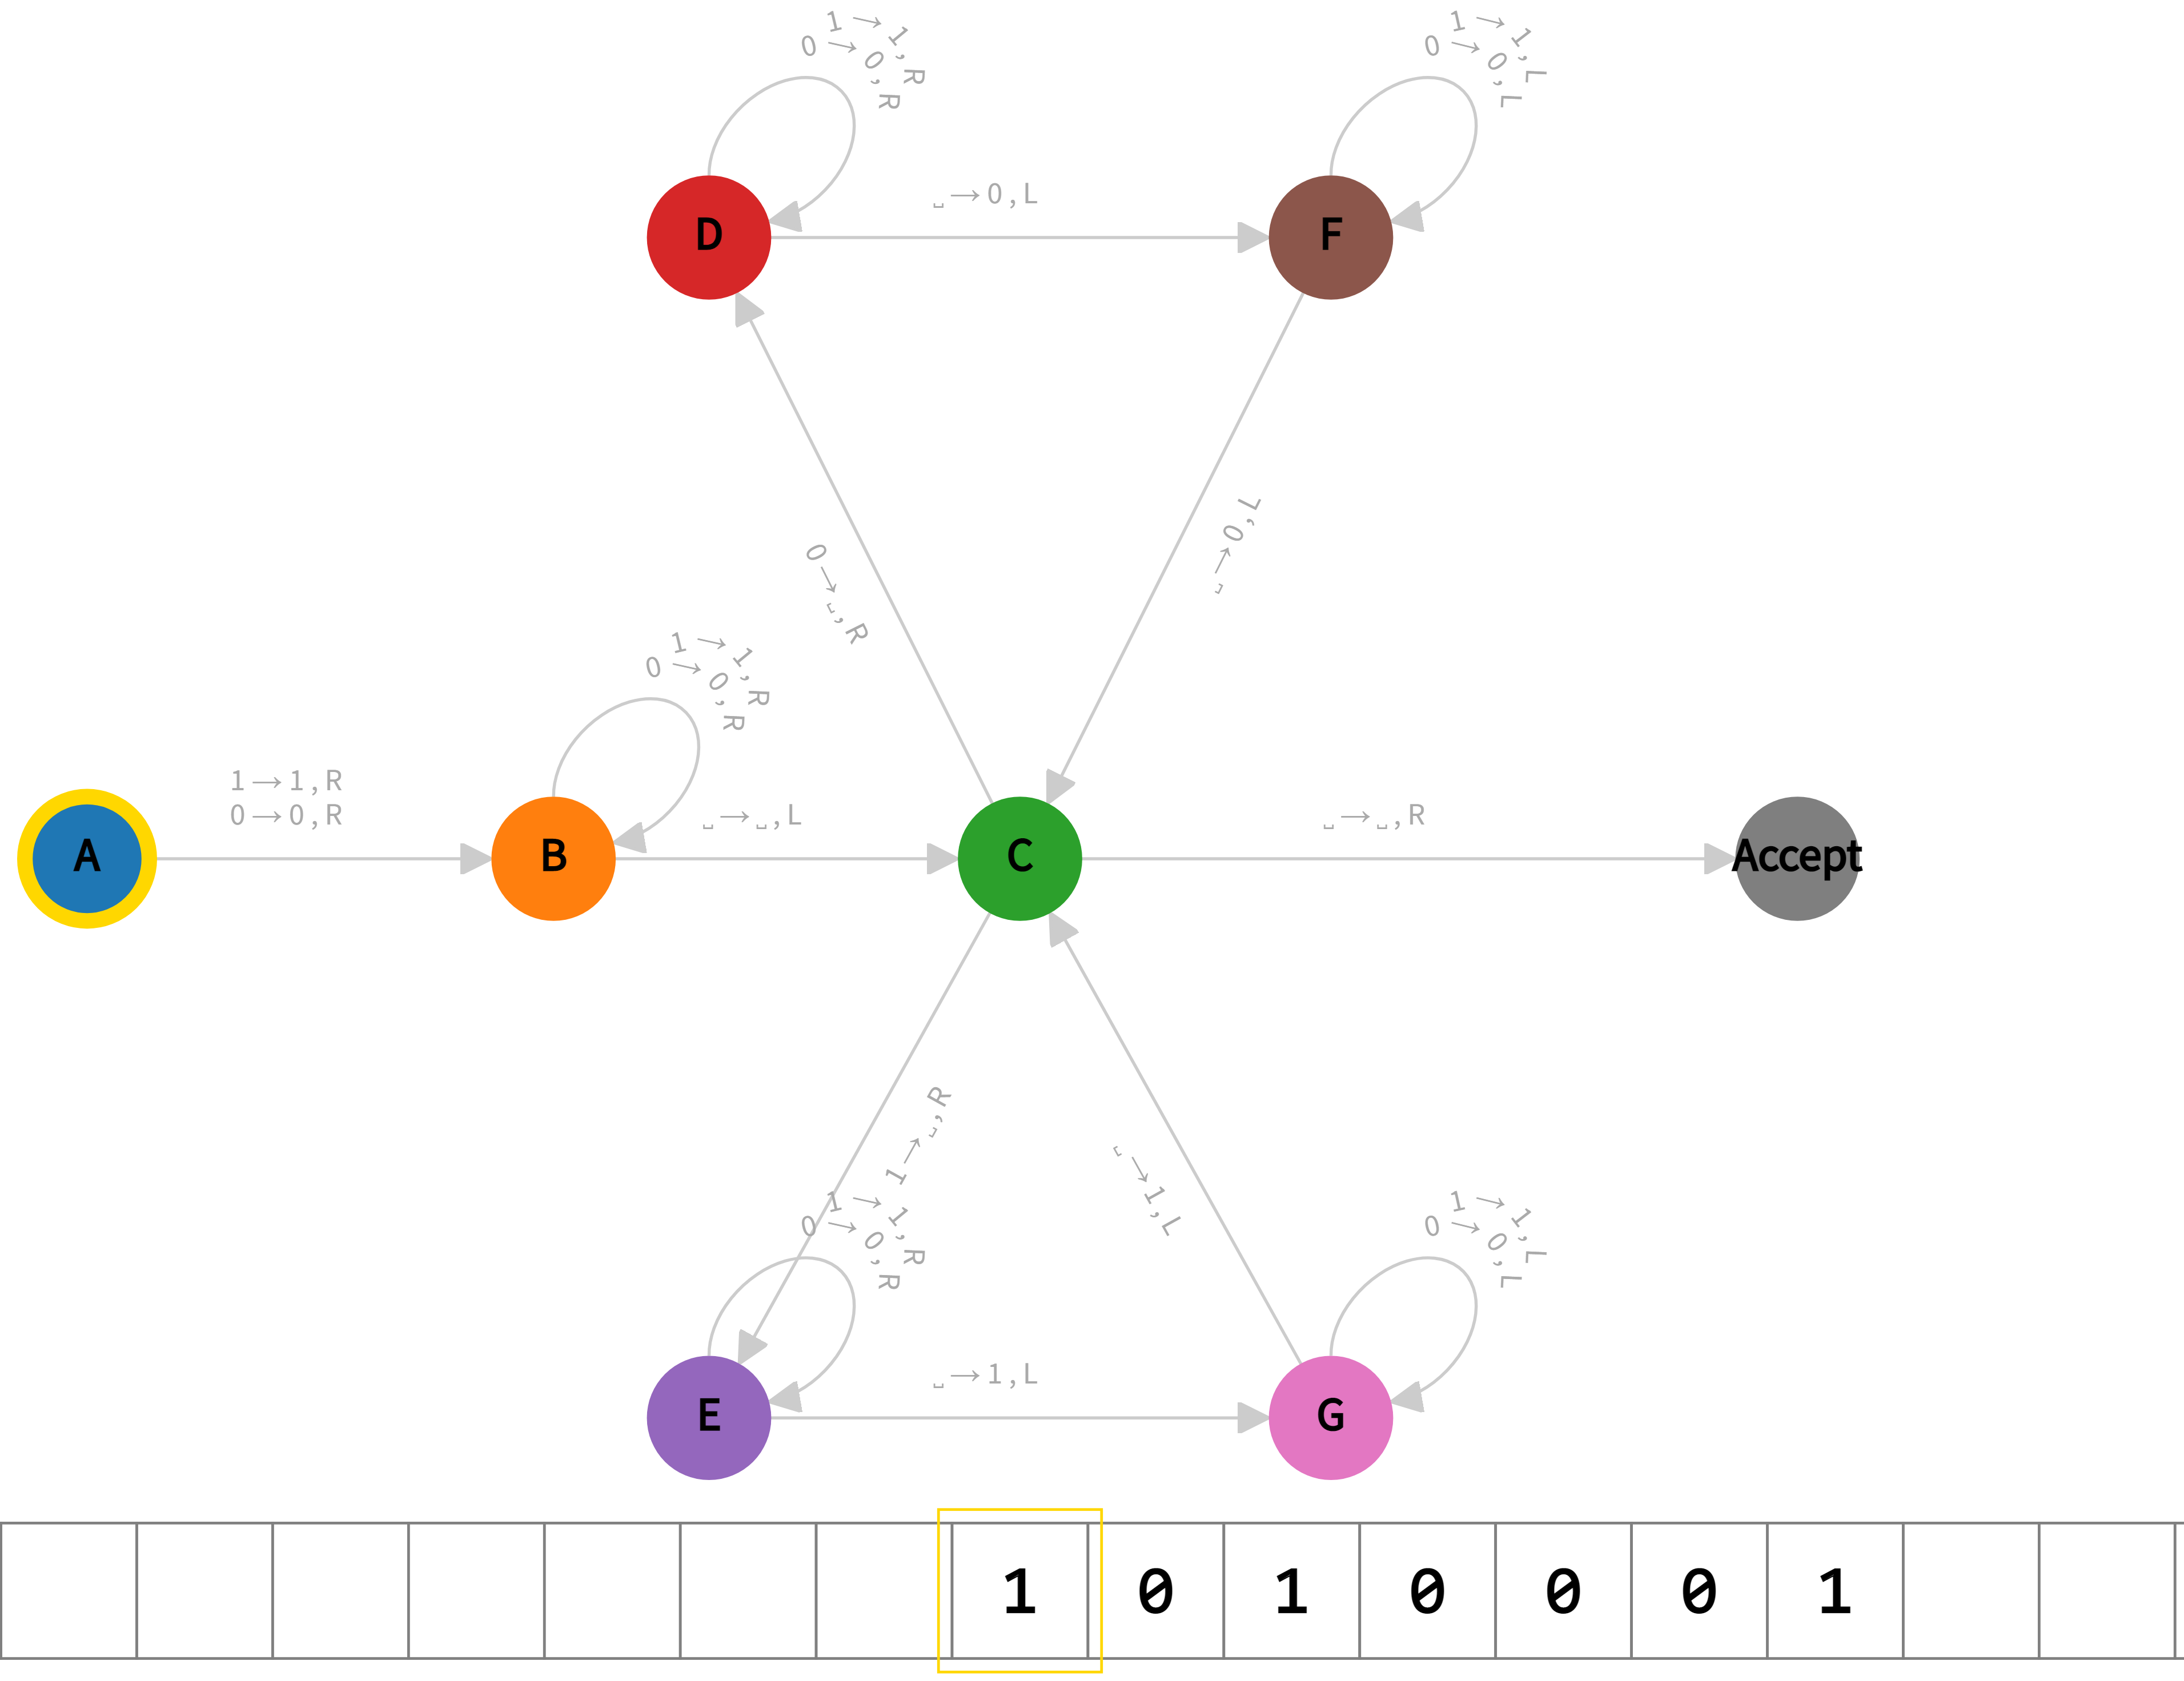
\includegraphics[width=\linewidth]{answers/img/q2-1010001-initial.png}
    \caption*{Figure (a): Initial State for $\mathbf{1010001}$}
    \label{fig:1010001-initial}
  \end{minipage}
  \begin{minipage}{.49\linewidth}
    \centering
    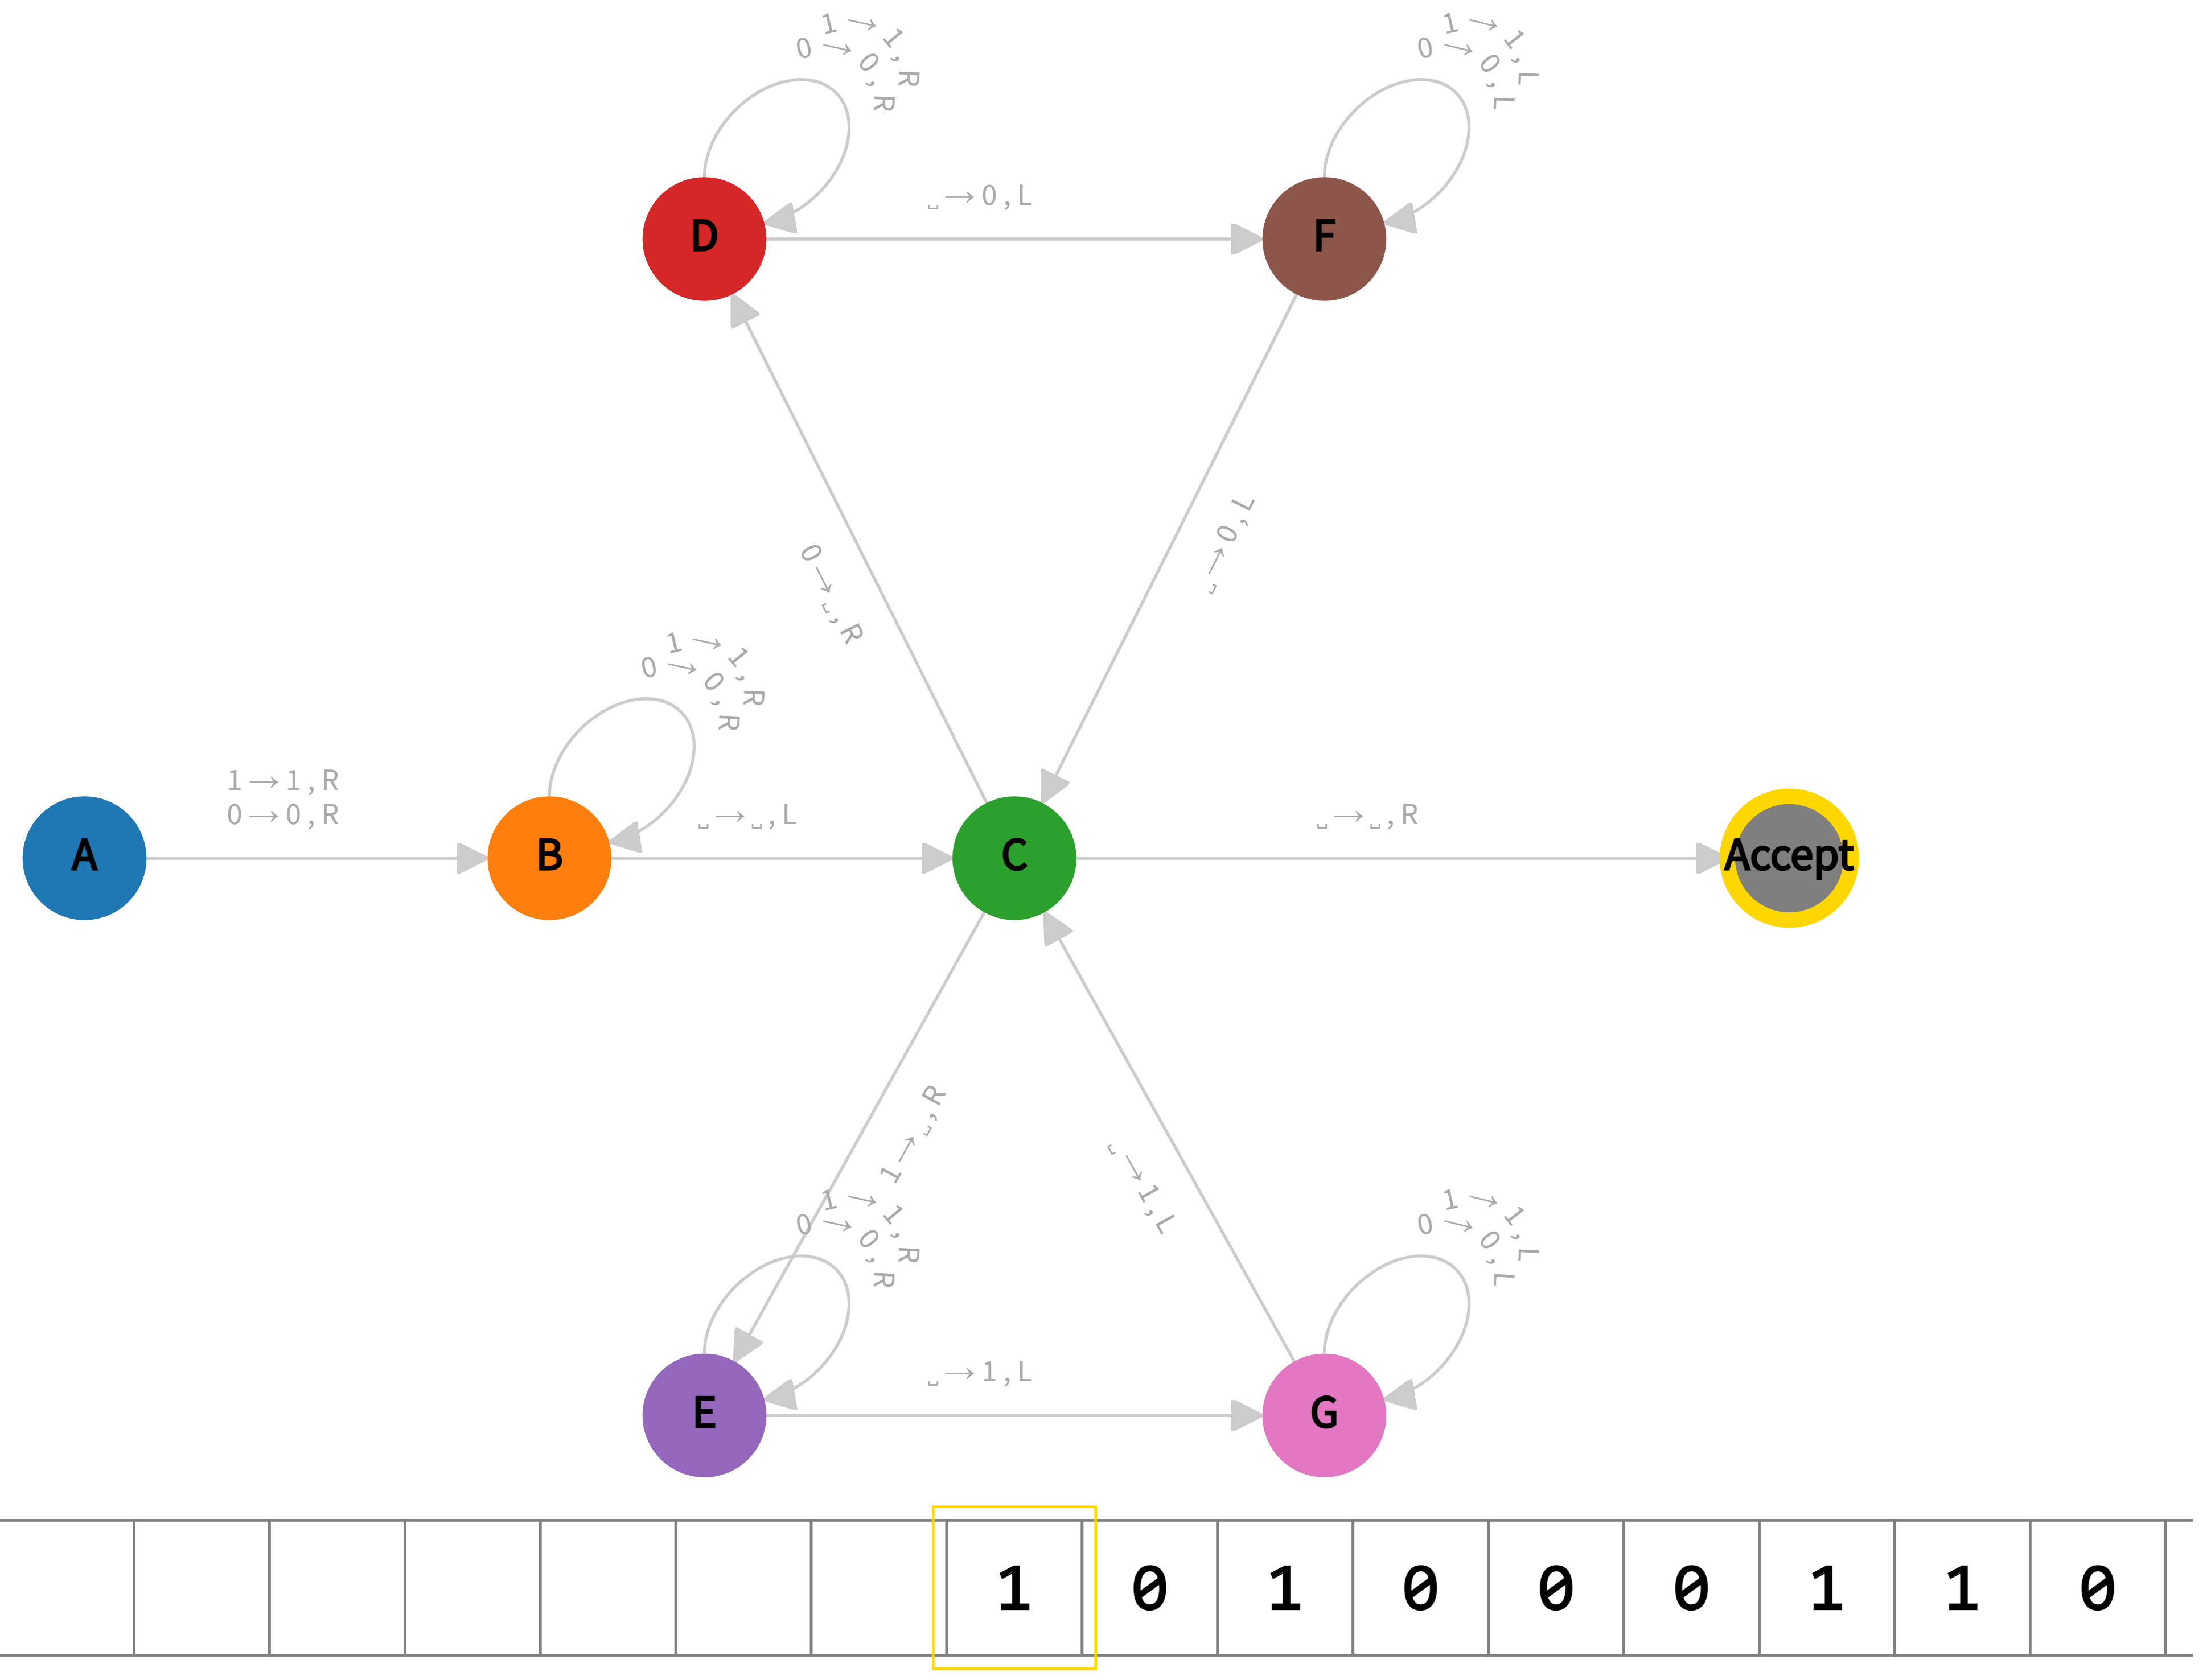
\includegraphics[width=\linewidth]{answers/img/q2-1010001-end.png}
    \caption*{Figure (b): End State for $\mathbf{1010001}$}
    \label{fig:1010001-end}
  \end{minipage}
  \caption{States for $\mathbf{1010001}$}
  \label{fig:in-1010001}
\end{figure}

\begin{center}
\textbf{\textit{Due to the head place, the whole output cannot be seen in \hyperref[fig:1010001-end]{Figure 13.b}.}}
\end{center}

\subsection*{Input: 00111}

\begin{figure}[ht]
  \centering
  \begin{minipage}{.49\linewidth}
    \centering
    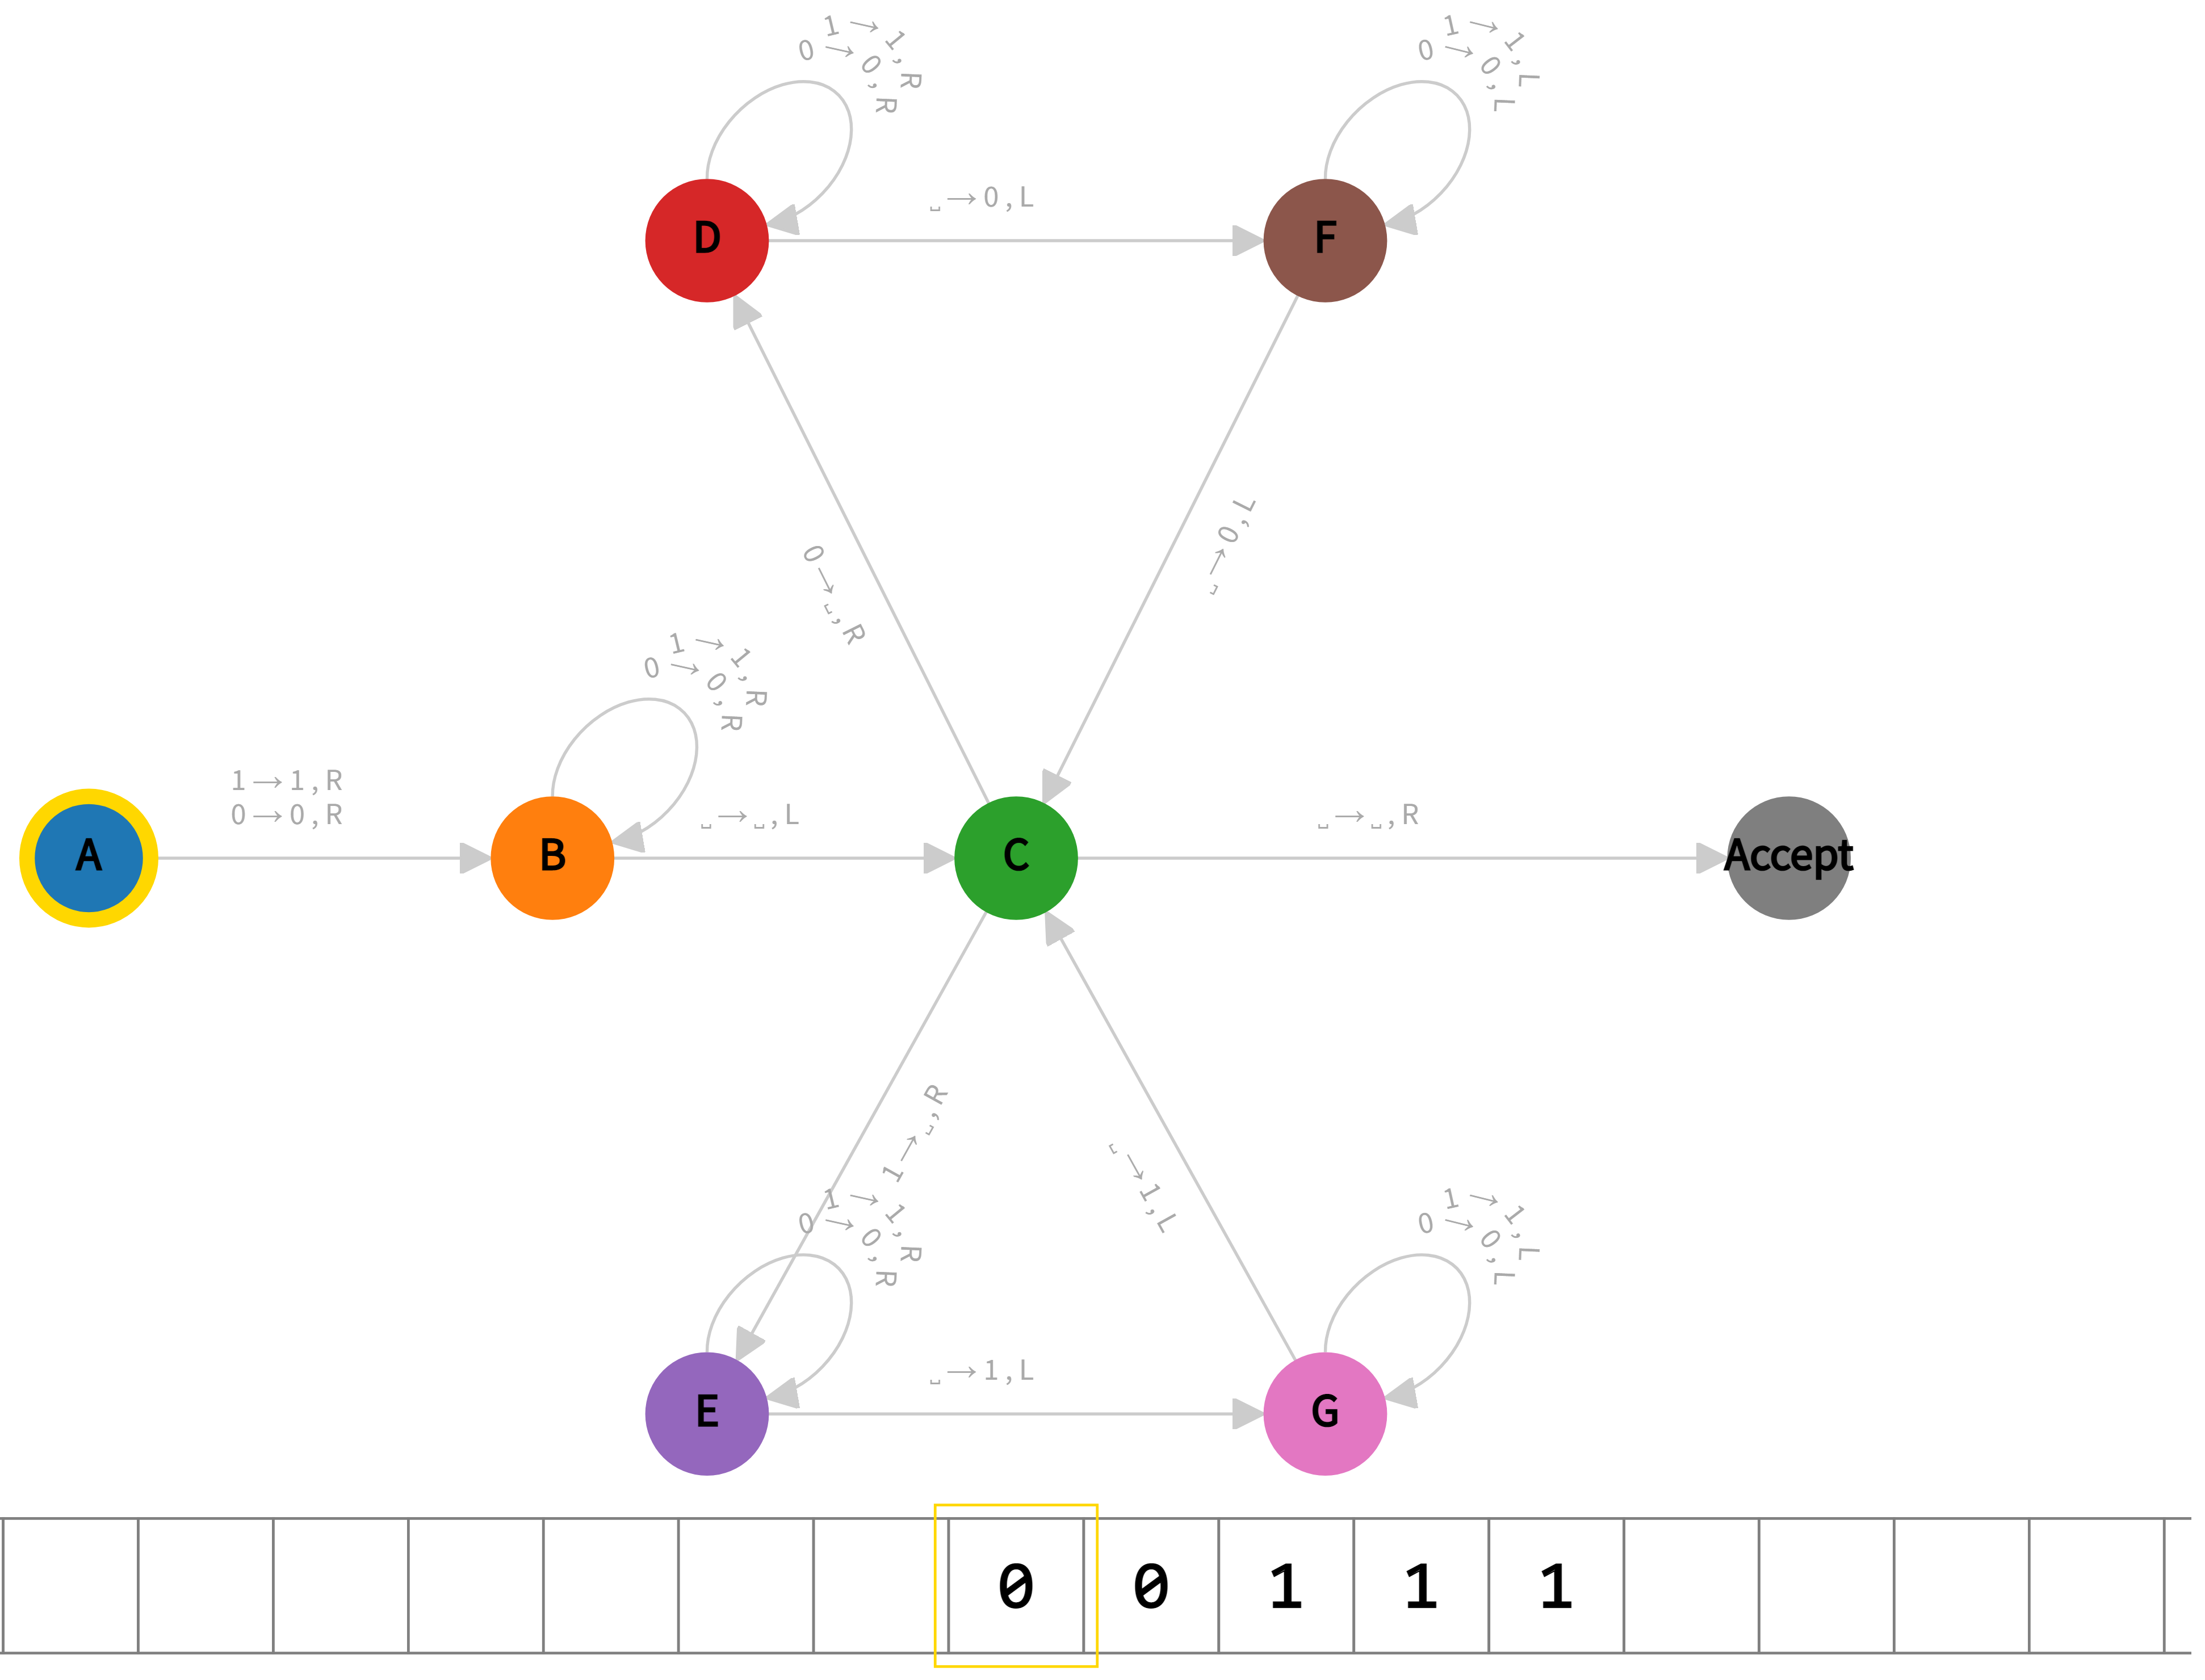
\includegraphics[width=\linewidth]{answers/img/q2-00111-initial.png}
    \caption*{Figure (a): Initial State for $\mathbf{00111}$}
    \label{fig:00111-initial}
  \end{minipage}
  \begin{minipage}{.49\linewidth}
    \centering
    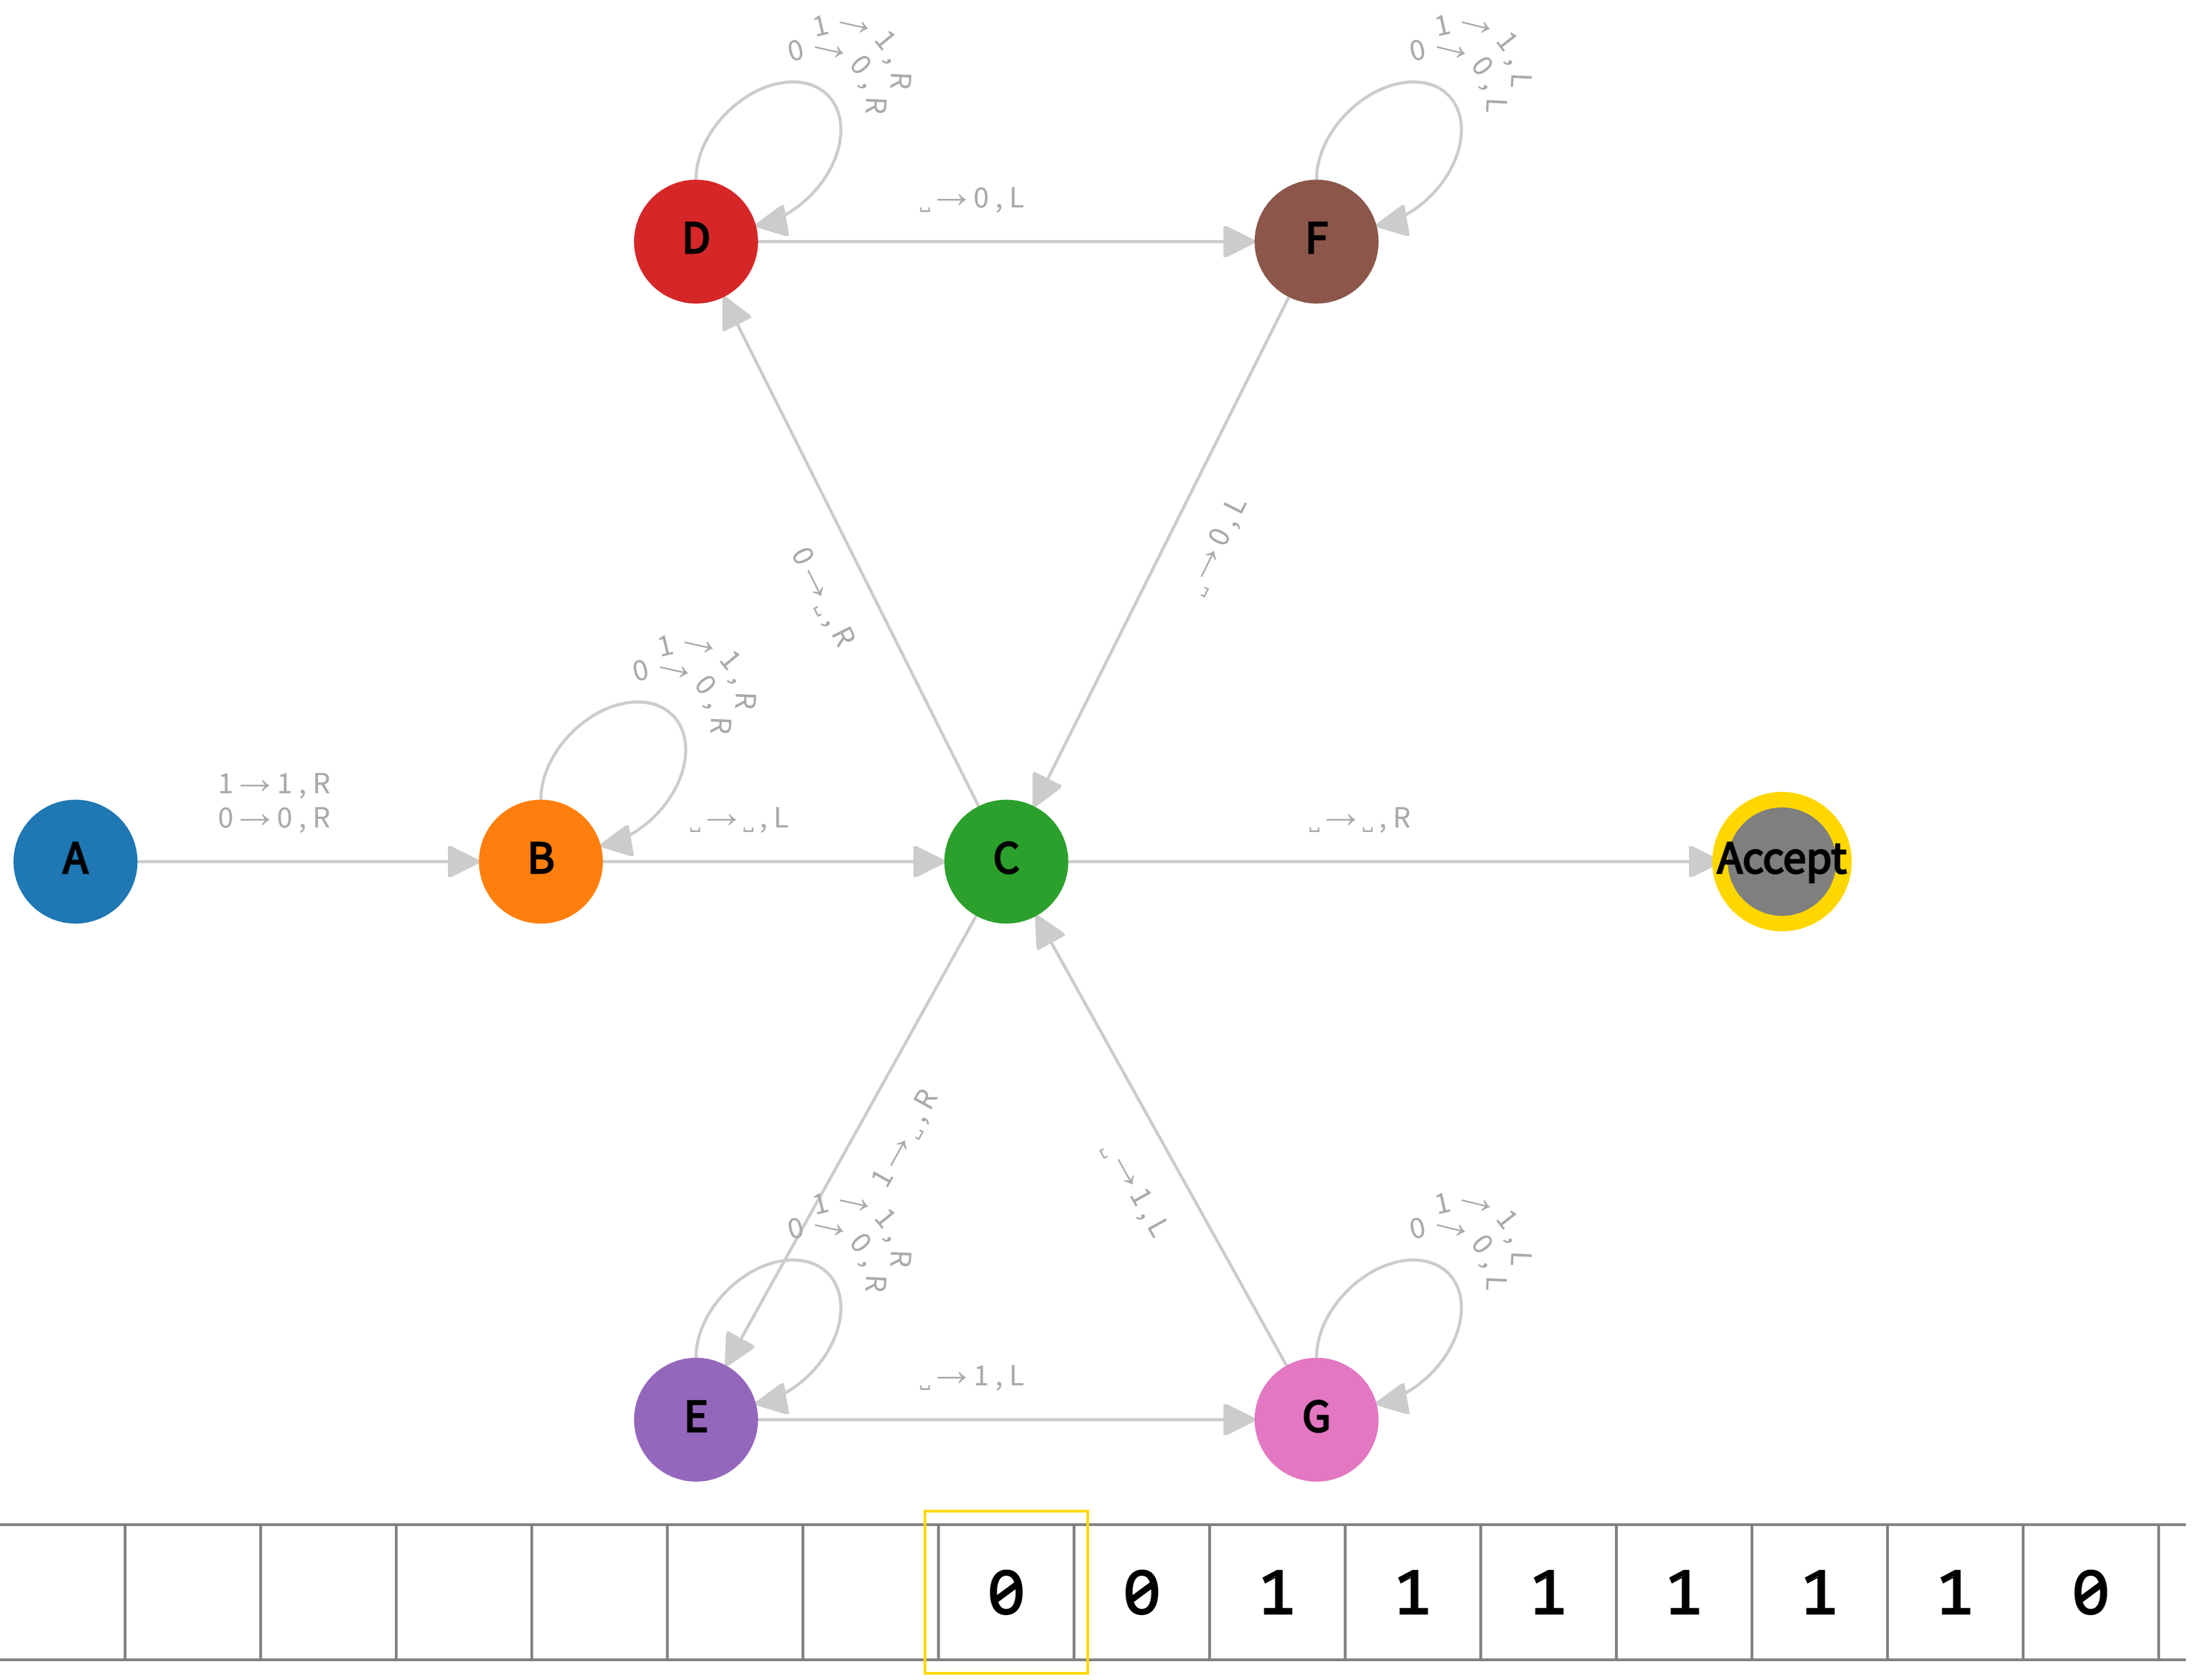
\includegraphics[width=\linewidth]{answers/img/q2-00111-end.png}
    \caption*{Figure (b): End State for $\mathbf{00111}$}
    \label{fig:00111-end}
  \end{minipage}
  \caption{States for $\mathbf{00111}$}
  \label{fig:in-00111}
\end{figure}

\begin{center}
\textbf{\textit{Due to the head place, the whole output cannot be seen in \hyperref[fig:00111-end]{Figure 14.b}.}}
\end{center}

\vspace*{\fill}
\newpage
